% \addtocontents{toc}{\protect\vspace{10pt}}
\appendix
\makeatletter
\renewcommand{\thesection}{\thechapter\@Alph\c@section}
\renewcommand{\thefigure}{\thesection.\arabic{figure}}
\renewcommand{\thetable}{\thesection.\arabic{table}}  
%\renewcommand{\thesubsection}{\thesection\@arabic\c@section}
%\renewcommand{\thesubsubsection}{\thesubsection\@arabic\c@section}
\makeatother

\chapter{Appendices}

\section{Other Bands}
\label{app:ps_sp_otherbands}

We present all the plots for the considered band ranges we analyzed during our experimental campaign setting the EER to be 0.0020 as discussed in Chapter~\ref{chap:ps_soundproof}.

\begin{figure}[!ht]
\centering
\subfigure[$B={[50\text{Hz}-630\text{Hz}]}$]{%
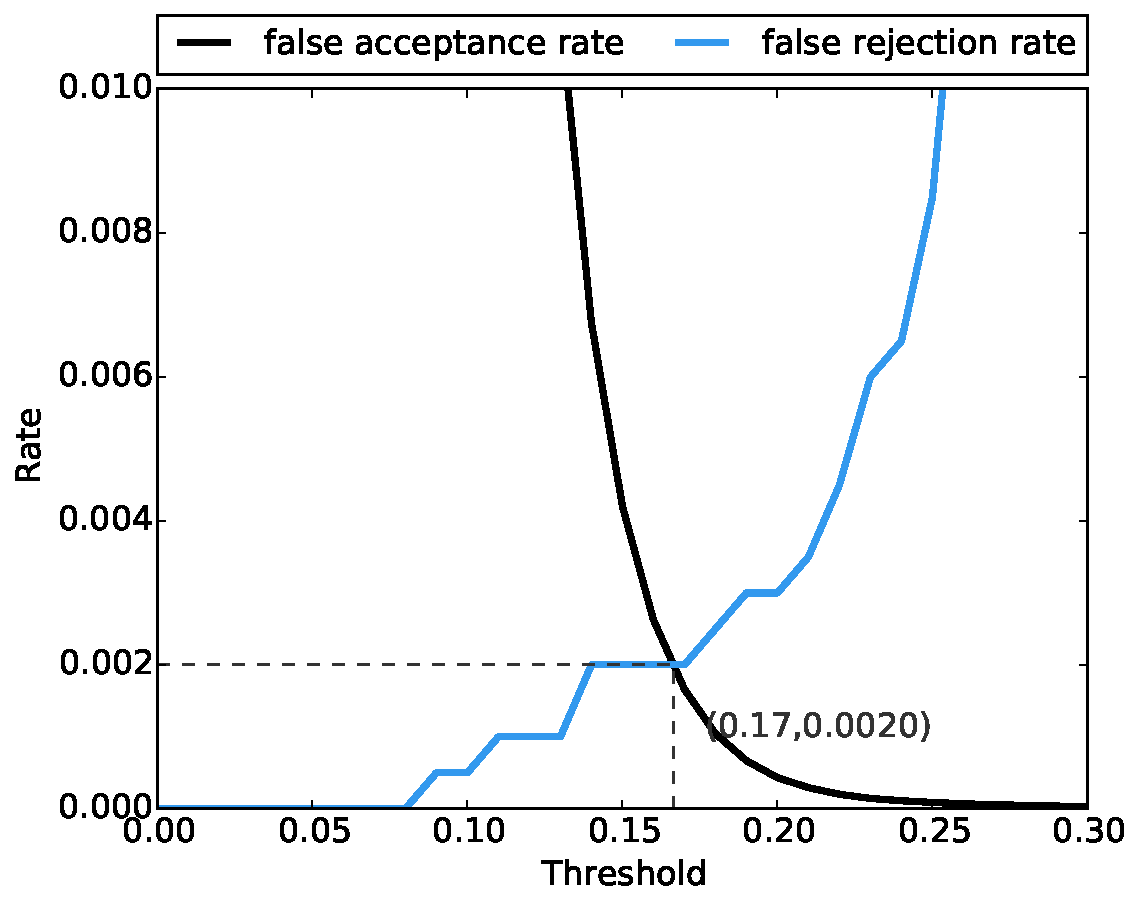
\includegraphics[width=.31\linewidth]{figures/appendix/falsepositives_50-630}}%
\subfigure[$B={[50\text{Hz}-800\text{Hz}]}$]{%
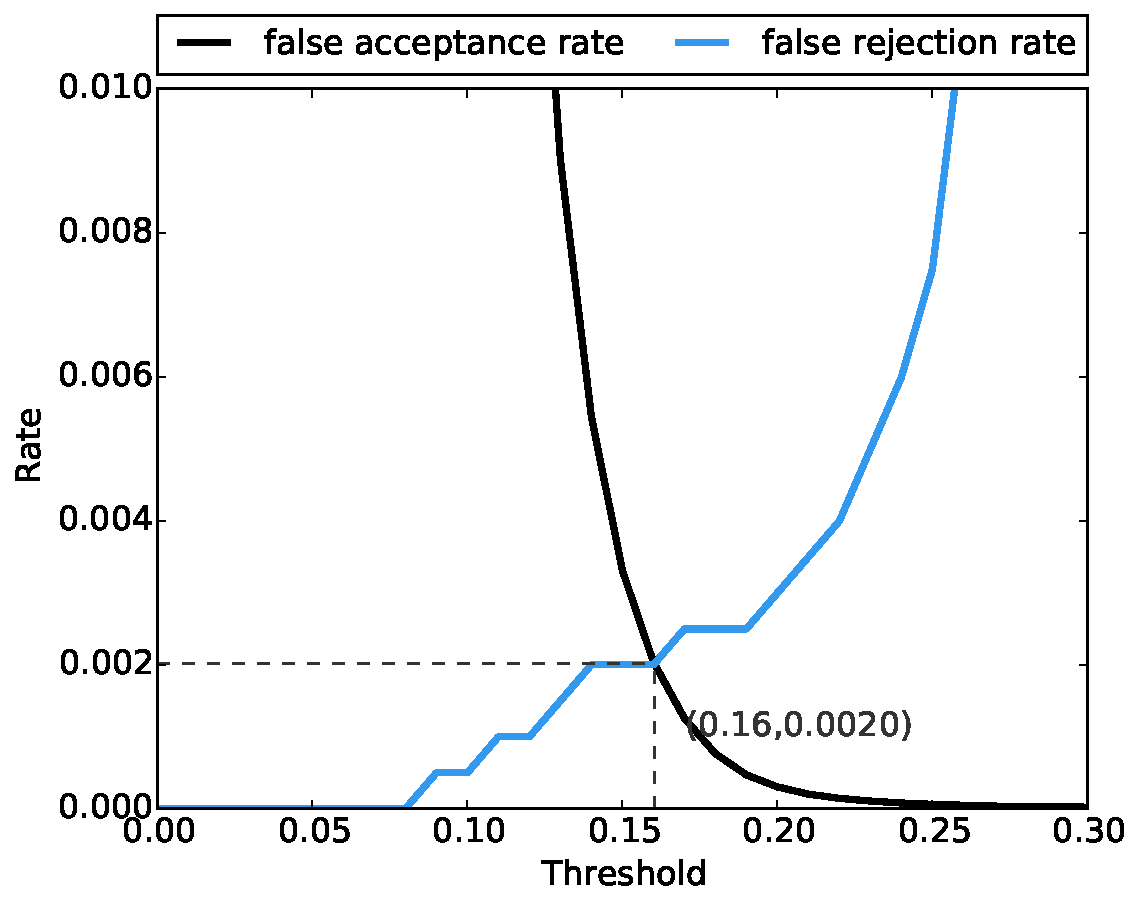
\includegraphics[width=.31\linewidth]{figures/appendix/falsepositives_50-800}}%
\subfigure[$B={[50\text{Hz}-1000\text{Hz}]}$]{%
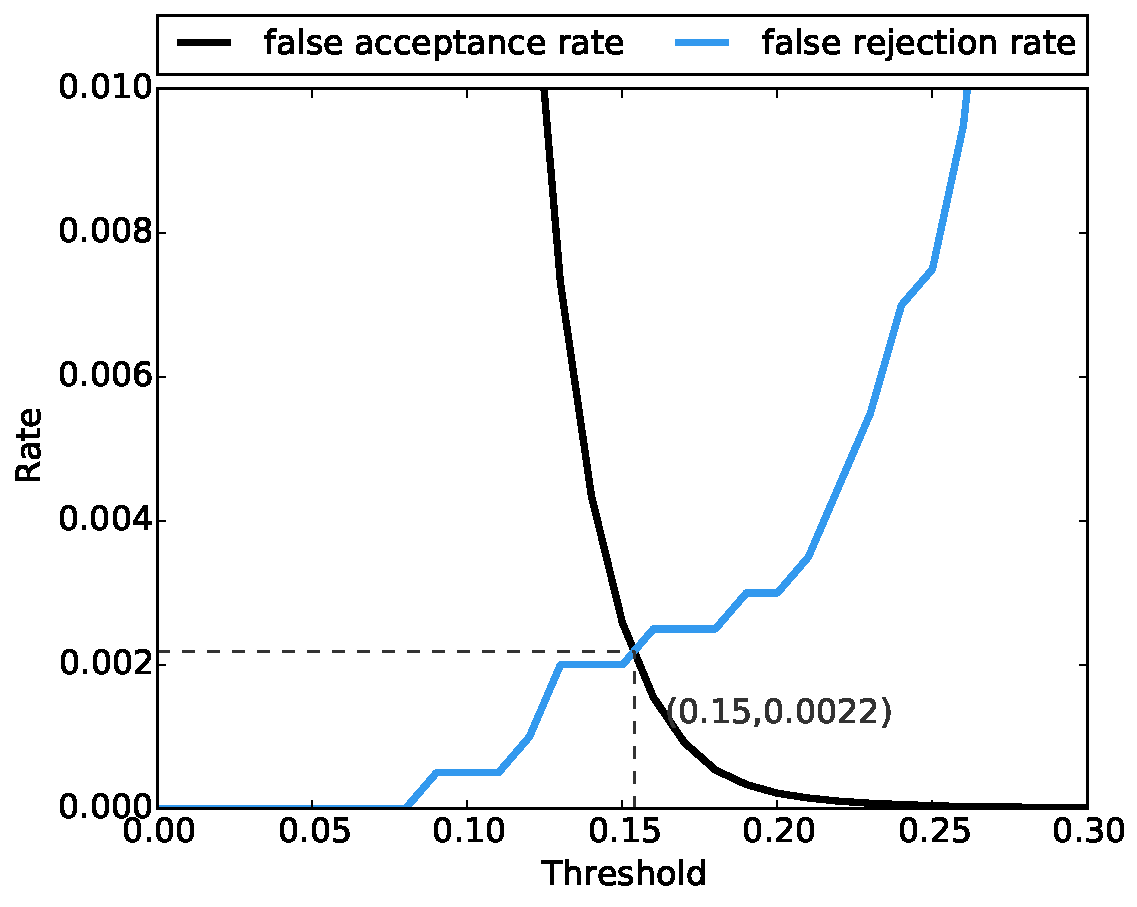
\includegraphics[width=.31\linewidth]{figures/appendix/falsepositives_50-1000}}%

\subfigure[$B={[50\text{Hz}-1250\text{Hz}]}$]{%
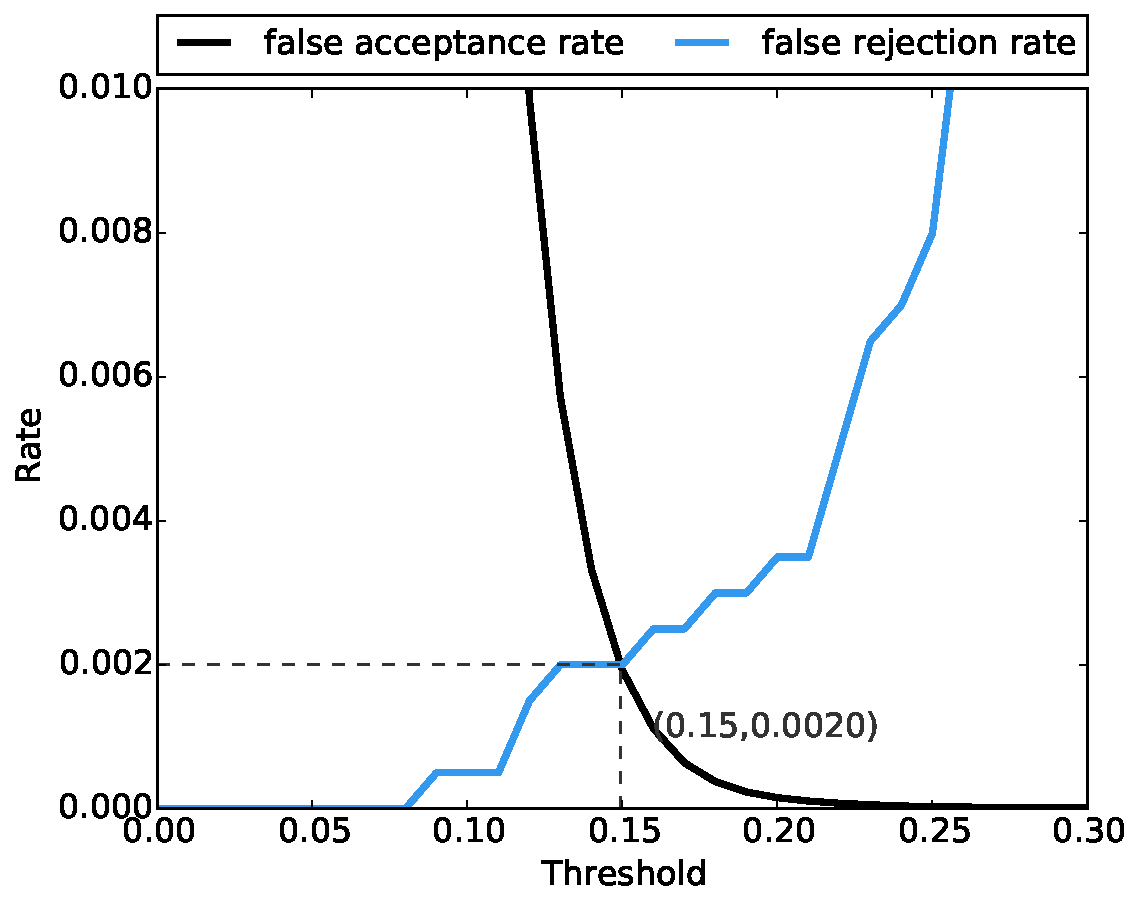
\includegraphics[width=.31\linewidth]{figures/appendix/falsepositives_50-1250}}%
\subfigure[$B={[50\text{Hz}-1600\text{Hz}]}$]{%
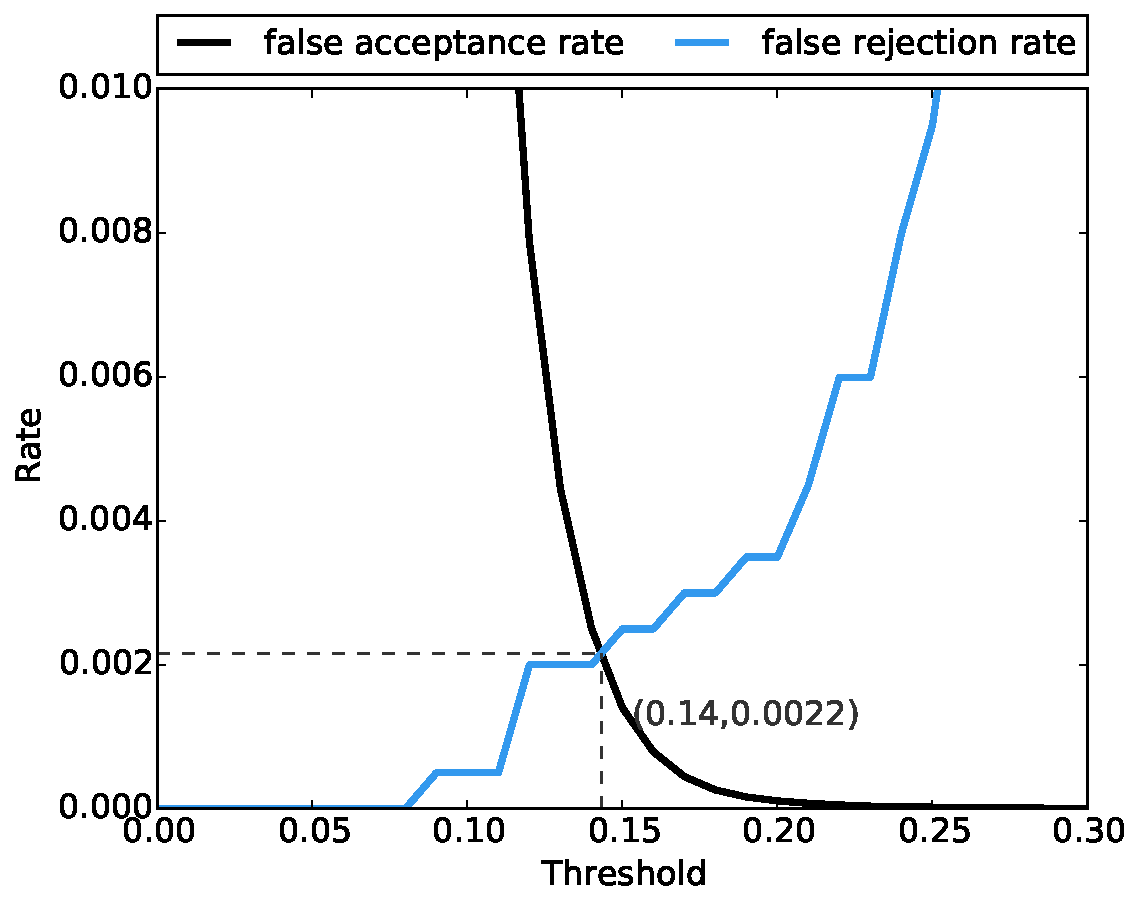
\includegraphics[width=.31\linewidth]{figures/appendix/falsepositives_50-1600}}%
\subfigure[$B={[50\text{Hz}-2000\text{Hz}]}$]{%
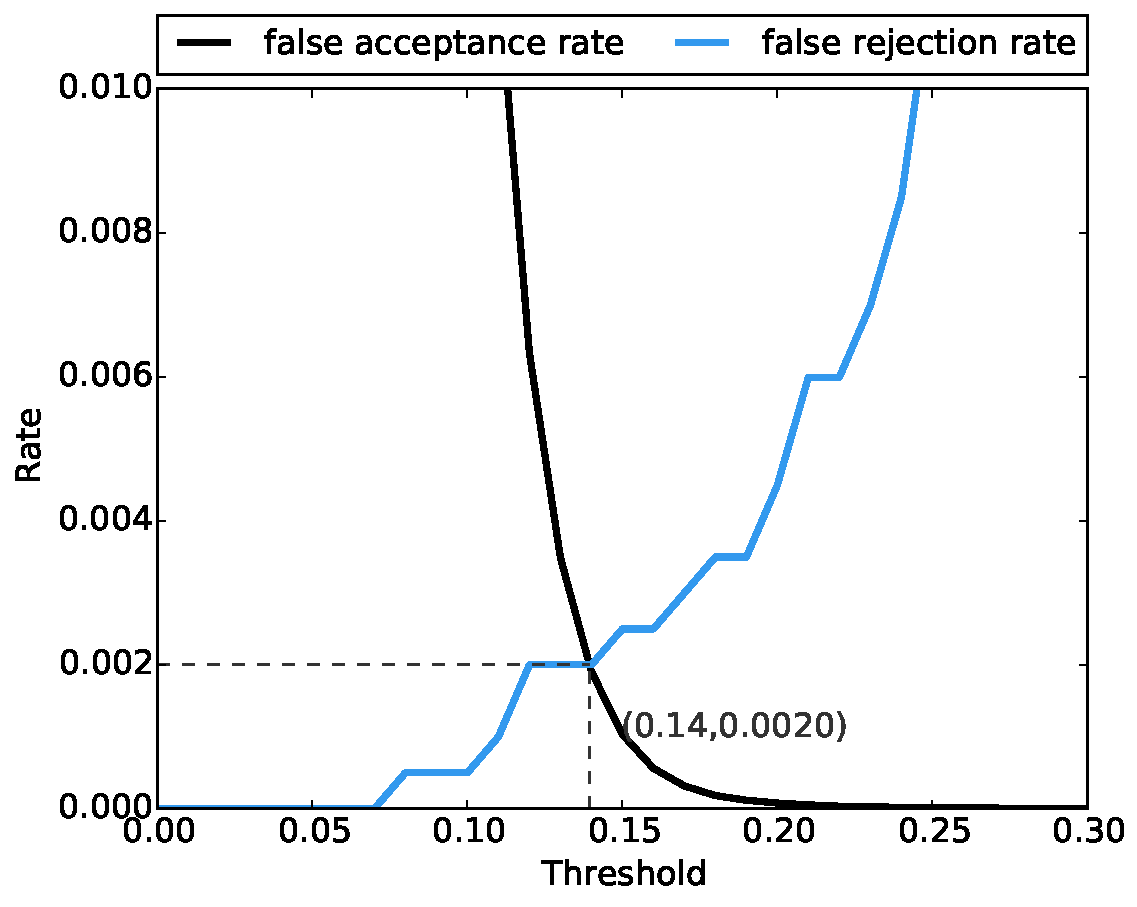
\includegraphics[width=.31\linewidth]{figures/appendix/falsepositives_50-2000}}%

\subfigure[$B={[50\text{Hz}-2500\text{Hz}]}$]{%
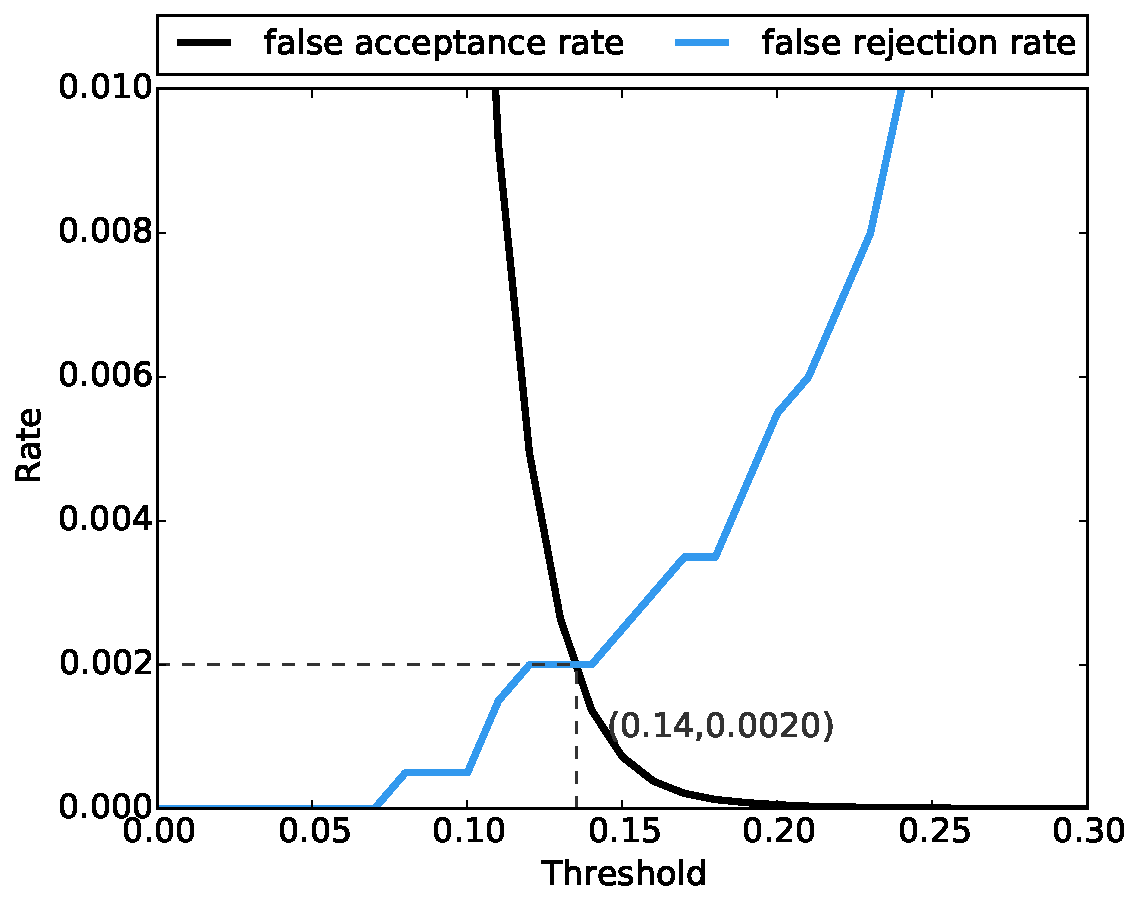
\includegraphics[width=.31\linewidth]{figures/appendix/falsepositives_50-2500}}%
\subfigure[$B={[50\text{Hz}-3150\text{Hz}]}$]{%
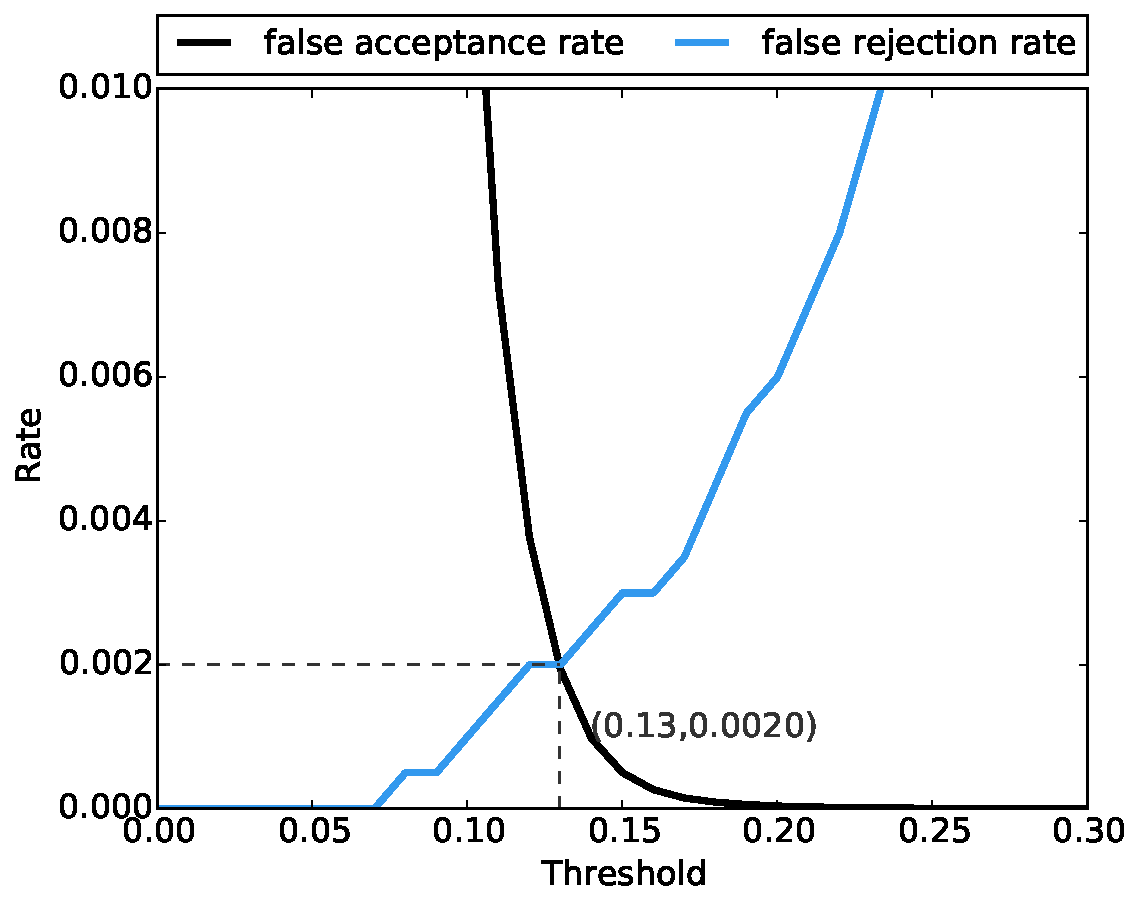
\includegraphics[width=.31\linewidth]{figures/appendix/falsepositives_50-3150}}%
\subfigure[$B={[50\text{Hz}-4000\text{Hz}]}$]{%
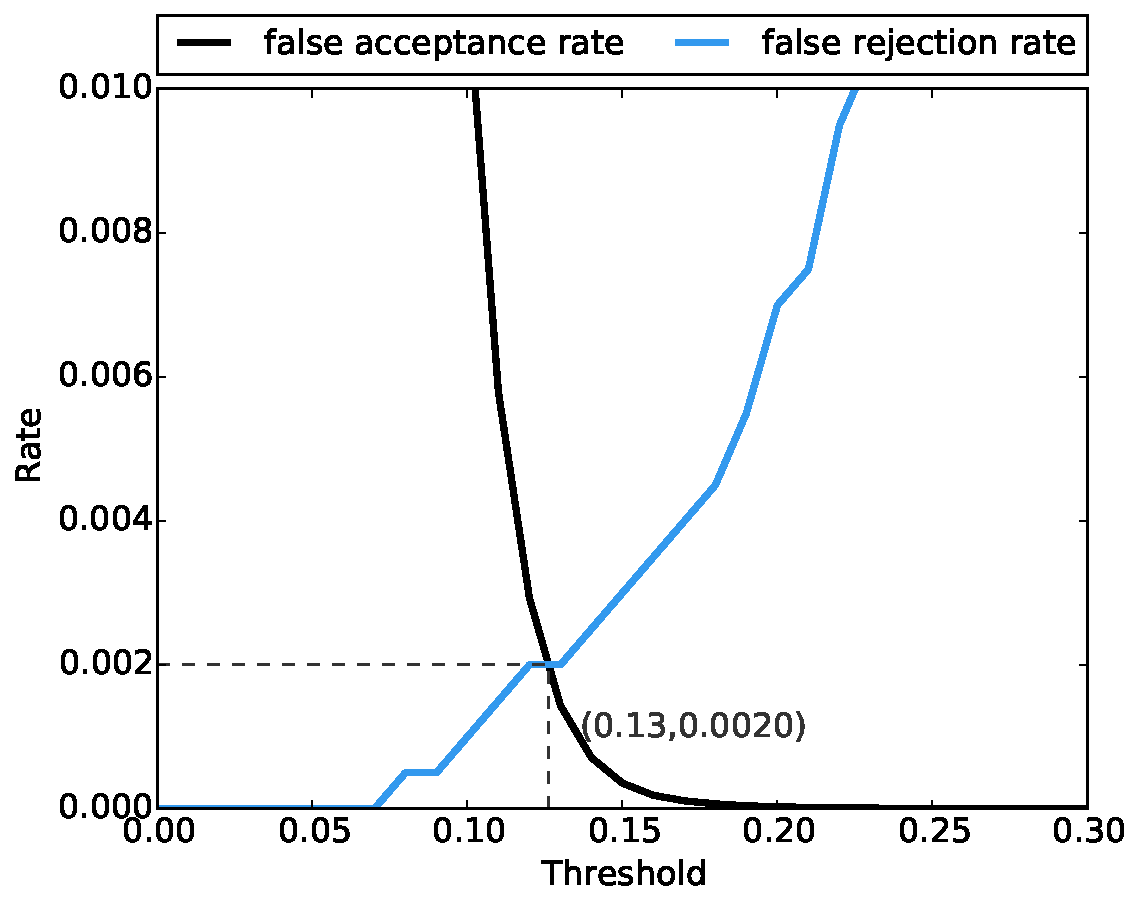
\includegraphics[width=.31\linewidth]{figures/appendix/falsepositives_50-4000}}%
\caption[{FRR and FAR as a function of the threshold $\tau_C$ for bands in the $B=[50\text{Hz}-[630\text{Hz}-4\text{kHz}]]$ range}]{False Rejection Rate and False Acceptance Rate as a function of the threshold $\tau_C$ for bands in the $B=[50\text{Hz}-[630\text{Hz}-4\text{kHz}]]$ range}
\end{figure}

\newpage

\begin{figure}[!ht]
\centering
\subfigure[$B={[63\text{Hz}-630\text{Hz}]}$]{%
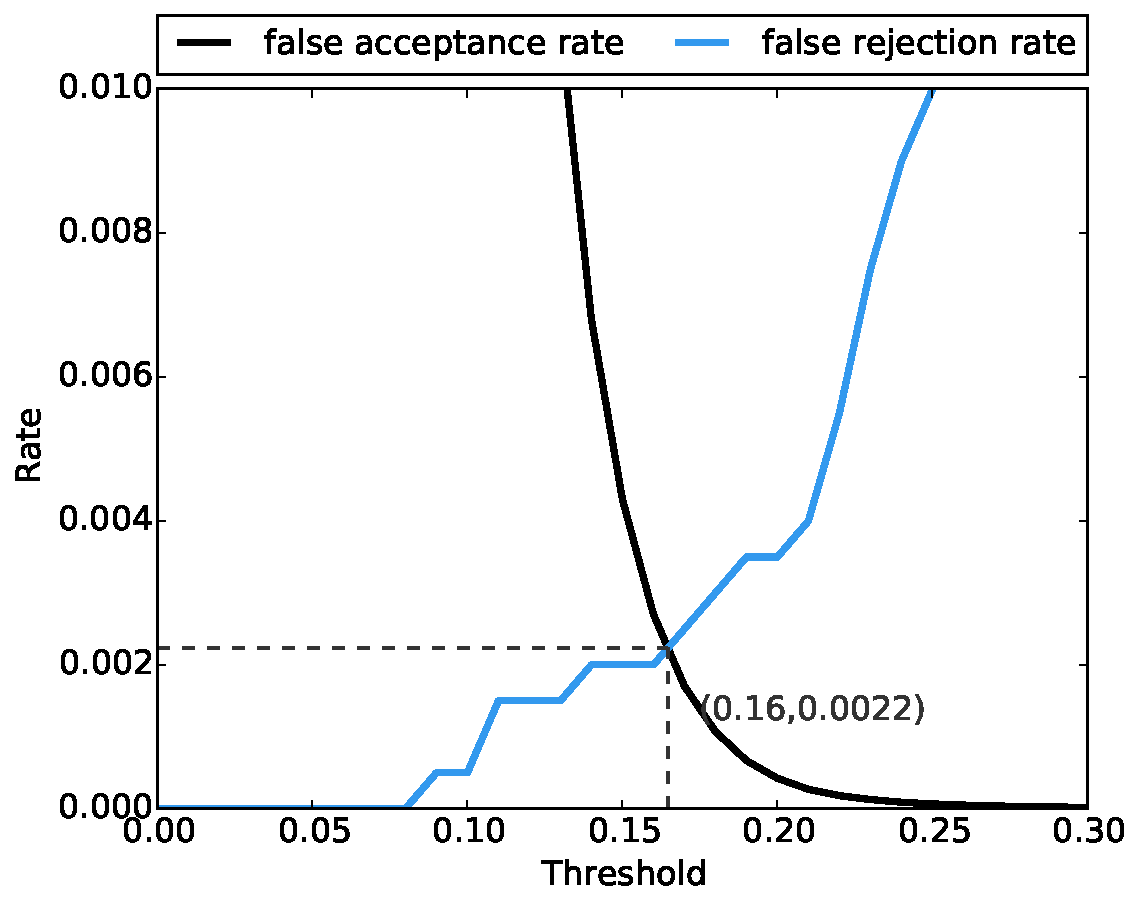
\includegraphics[width=.31\linewidth]{figures/appendix/falsepositives_63-630}}%
\subfigure[$B={[63\text{Hz}-800\text{Hz}]}$]{%
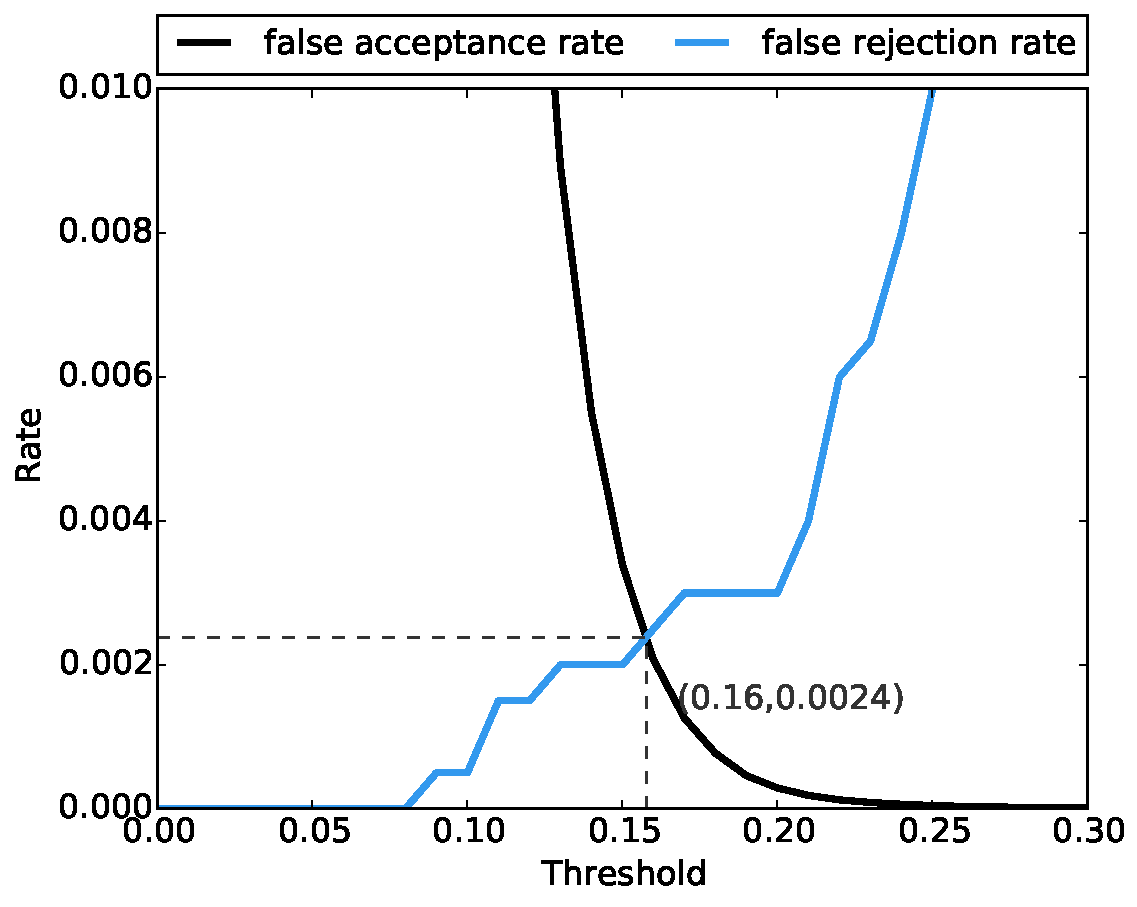
\includegraphics[width=.31\linewidth]{figures/appendix/falsepositives_63-800}}%
\subfigure[$B={[63\text{Hz}-1000\text{Hz}]}$]{%
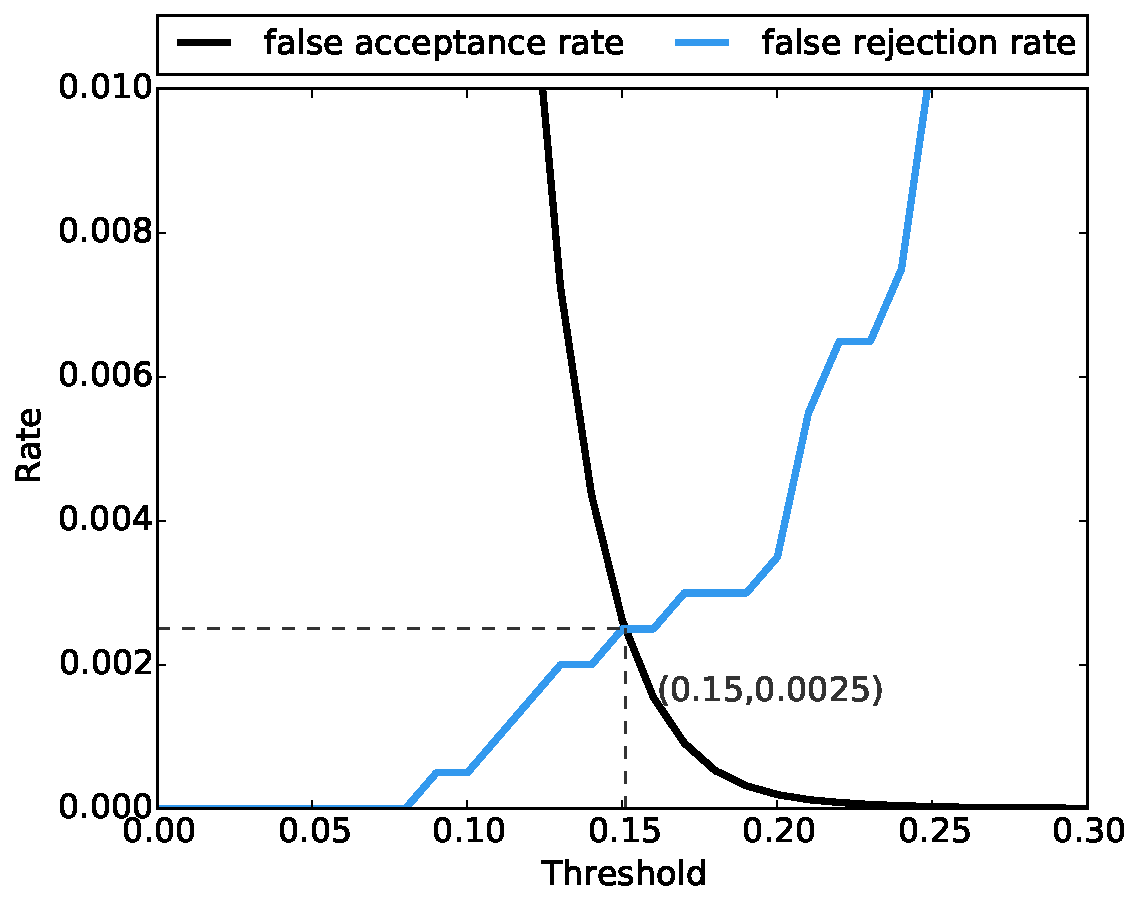
\includegraphics[width=.31\linewidth]{figures/appendix/falsepositives_63-1000}}%

\subfigure[$B={[63\text{Hz}-1250\text{Hz}]}$]{%
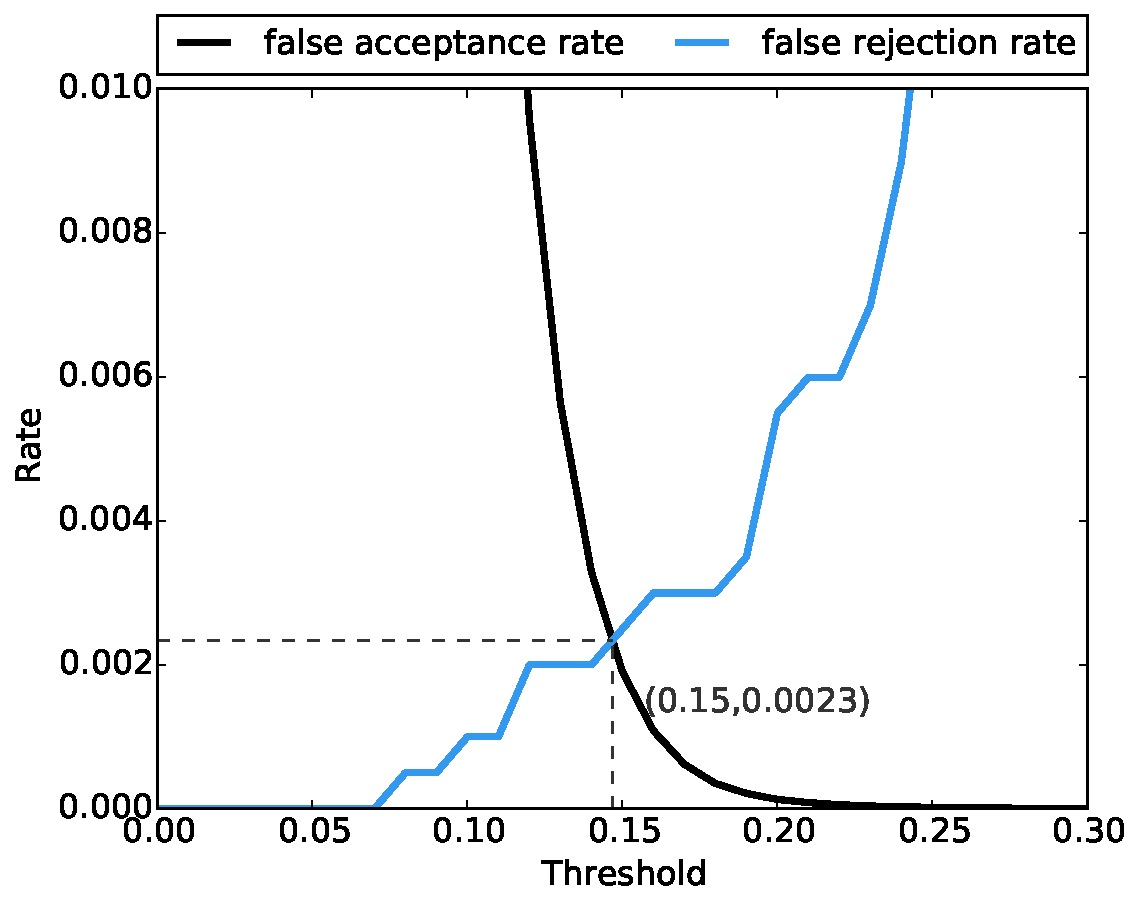
\includegraphics[width=.31\linewidth]{figures/appendix/falsepositives_63-1250}}%
\subfigure[$B={[63\text{Hz}-1600\text{Hz}]}$]{%
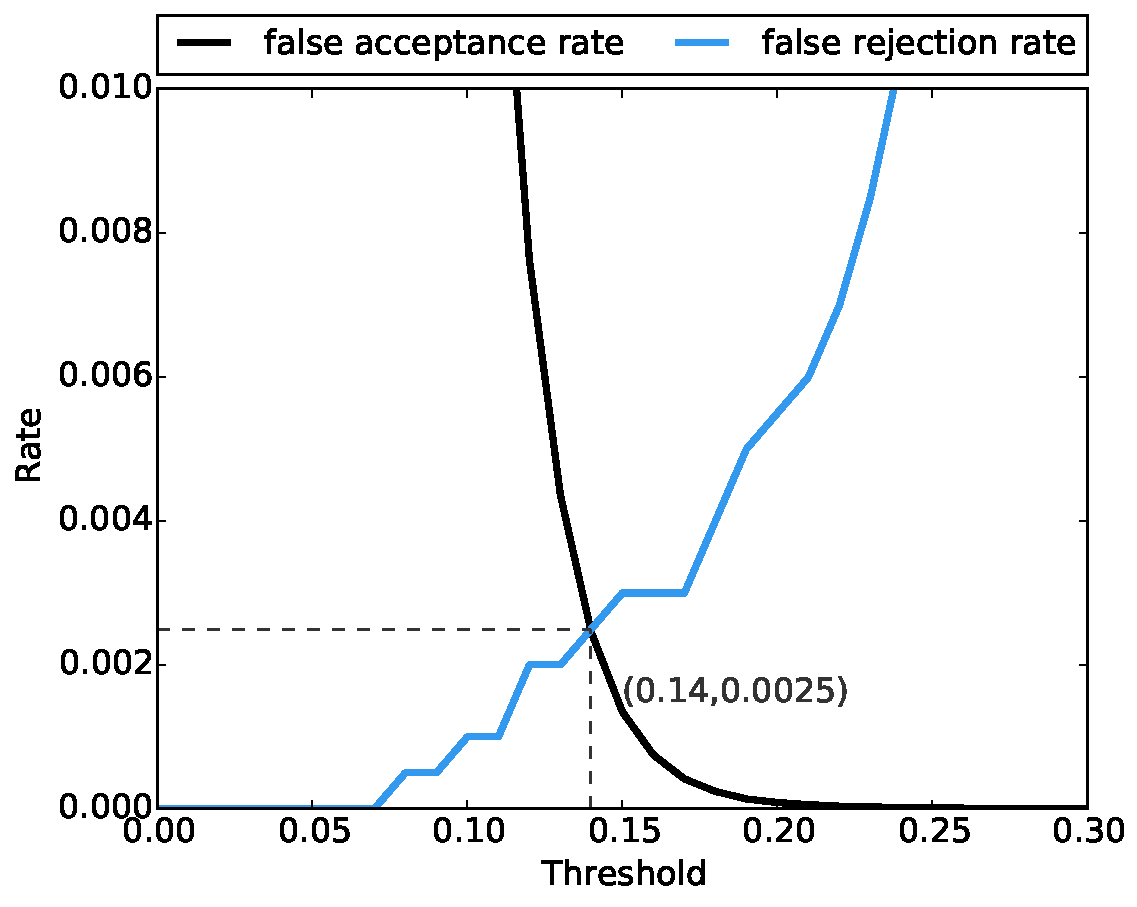
\includegraphics[width=.31\linewidth]{figures/appendix/falsepositives_63-1600}}%
\subfigure[$B={[63\text{Hz}-2000\text{Hz}]}$]{%
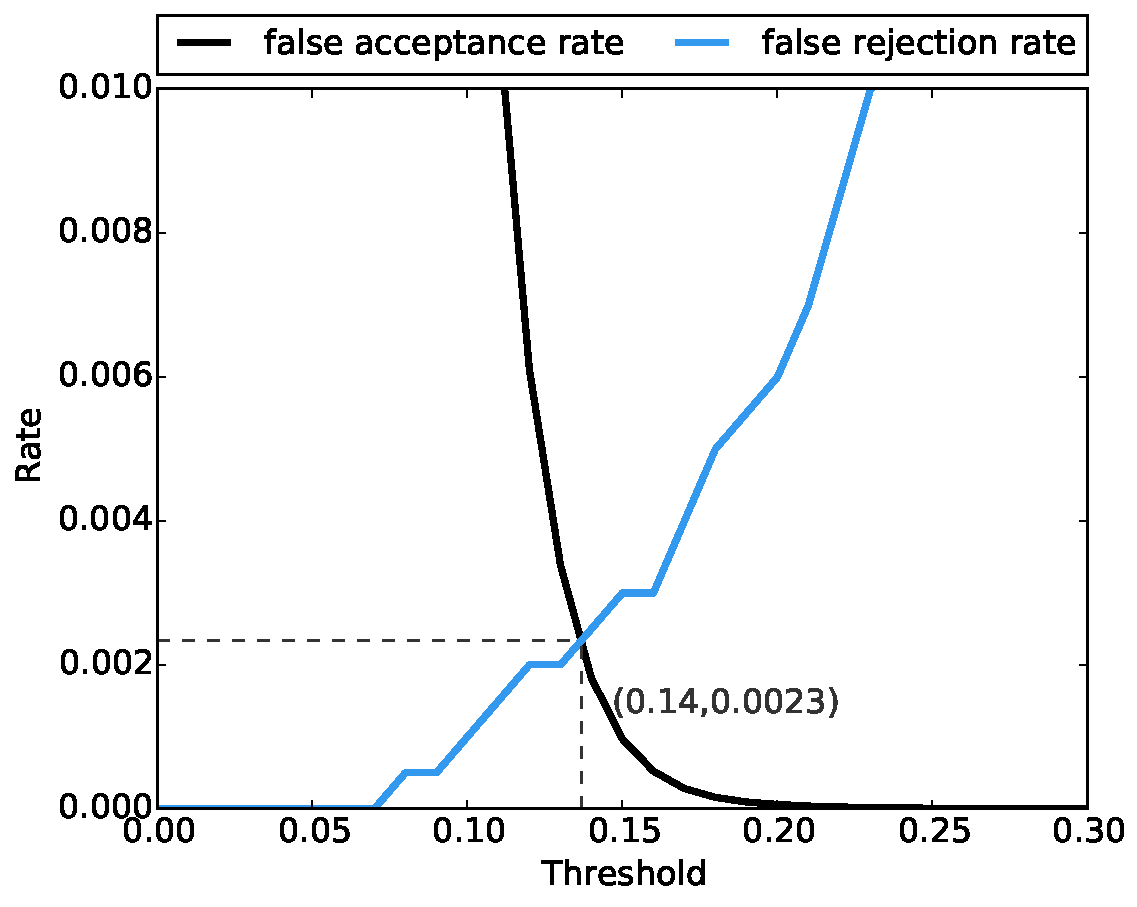
\includegraphics[width=.31\linewidth]{figures/appendix/falsepositives_63-2000}}%

\subfigure[$B={[63\text{Hz}-2500\text{Hz}]}$]{%
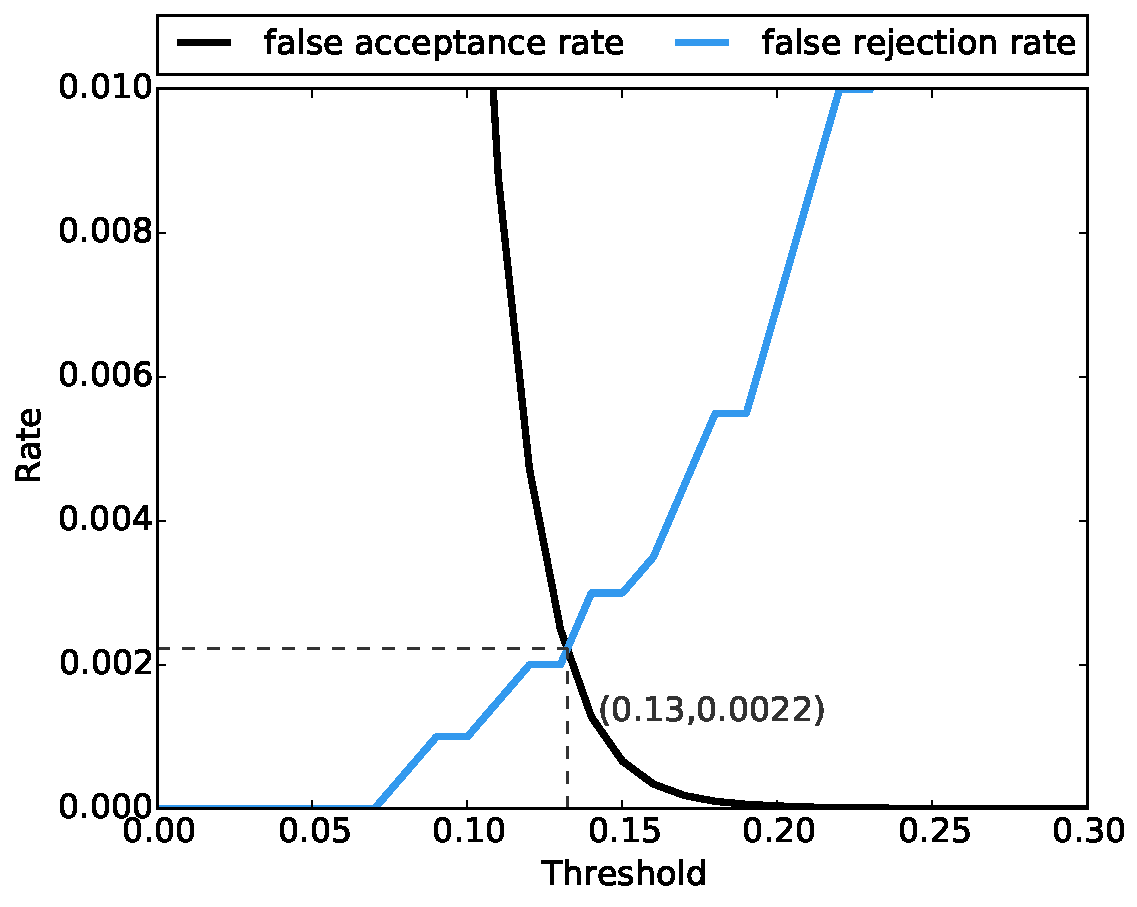
\includegraphics[width=.31\linewidth]{figures/appendix/falsepositives_63-2500}}%
\subfigure[$B={[63\text{Hz}-3150\text{Hz}]}$]{%
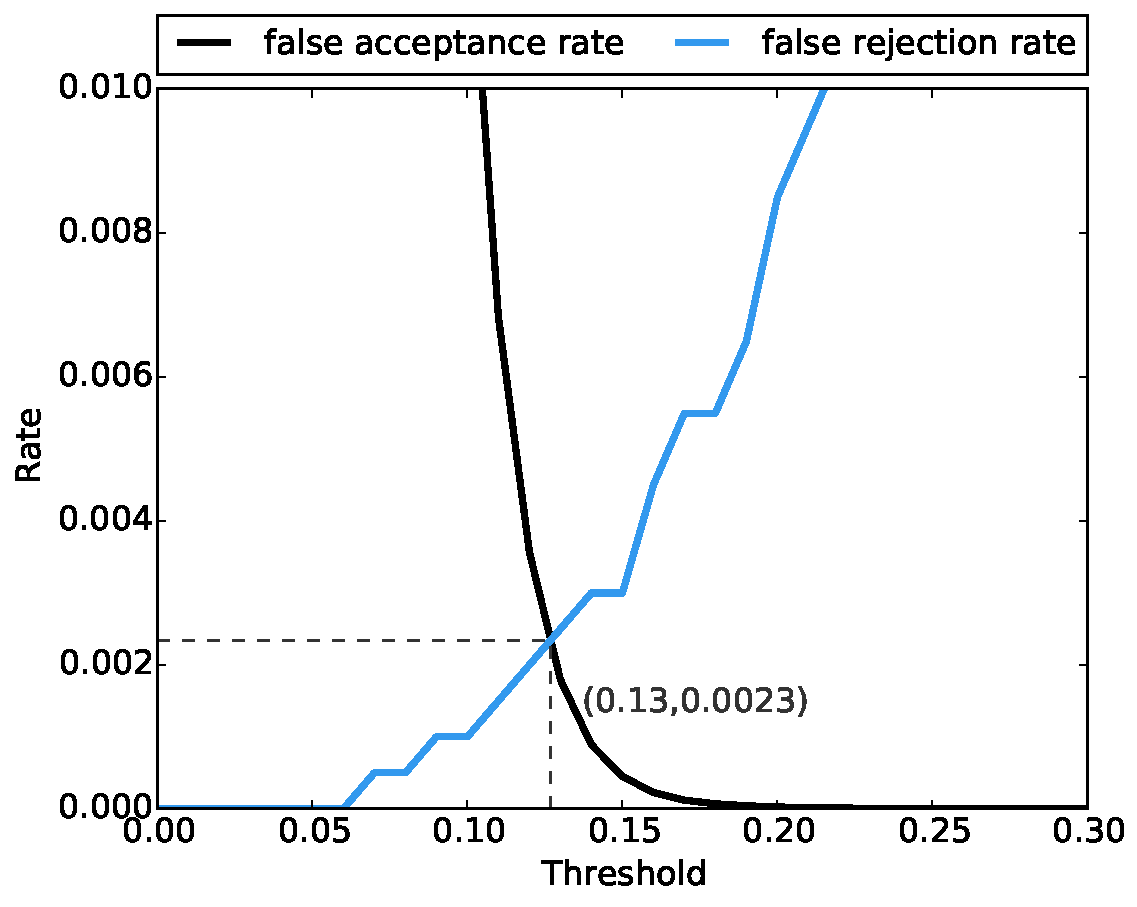
\includegraphics[width=.31\linewidth]{figures/appendix/falsepositives_63-3150}}%
\subfigure[$B={[63\text{Hz}-4000\text{Hz}]}$]{%
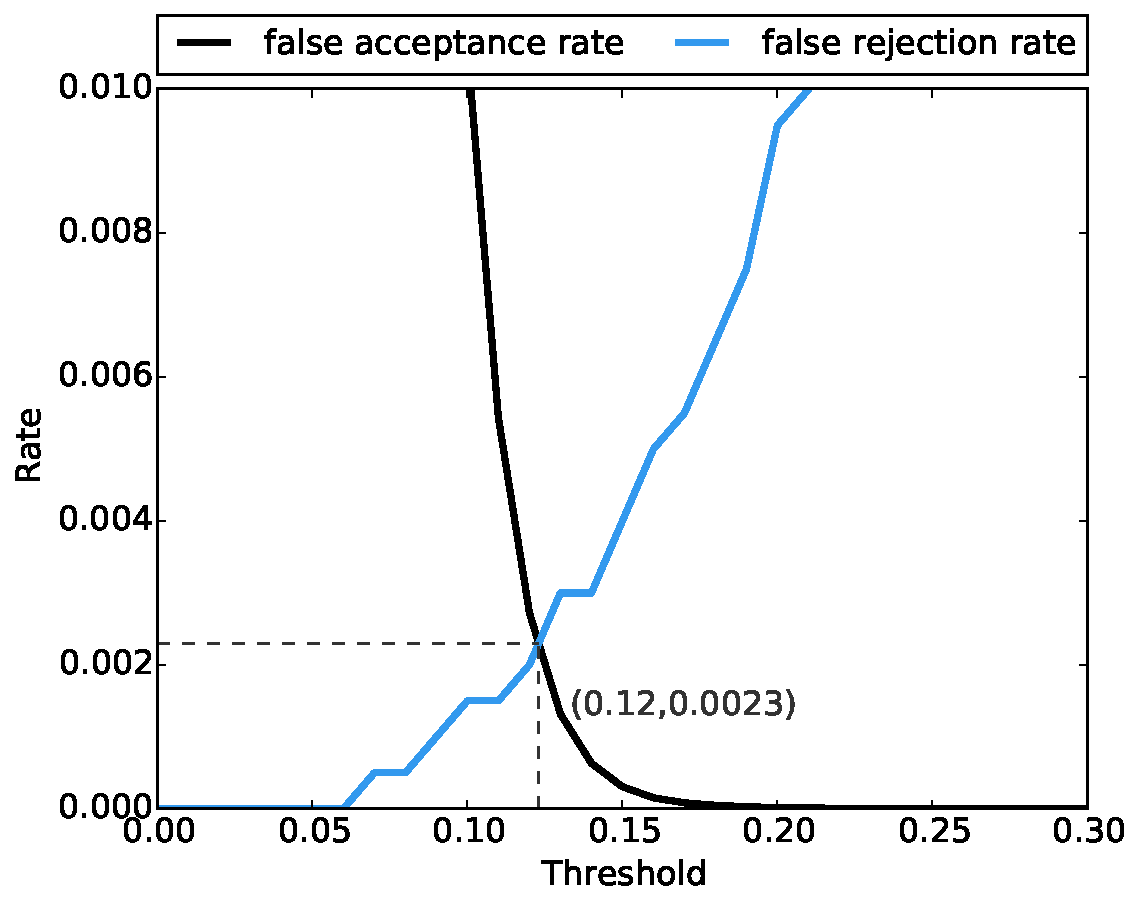
\includegraphics[width=.31\linewidth]{figures/appendix/falsepositives_63-4000}}%
\caption[{FRR and FAR as a function of the threshold $\tau_C$ for bands in the $B=[63\text{Hz}-[630\text{Hz}-4\text{kHz}]]$ range}]{False Rejection Rate and False Acceptance Rate as a function of the threshold $\tau_C$ for bands in the $B=[63\text{Hz}-[630\text{Hz}-4\text{kHz}]]$ range}
\end{figure}

\newpage

\begin{figure}[!ht]
\centering
\subfigure[$B={[80\text{Hz}-630\text{Hz}]}$]{%
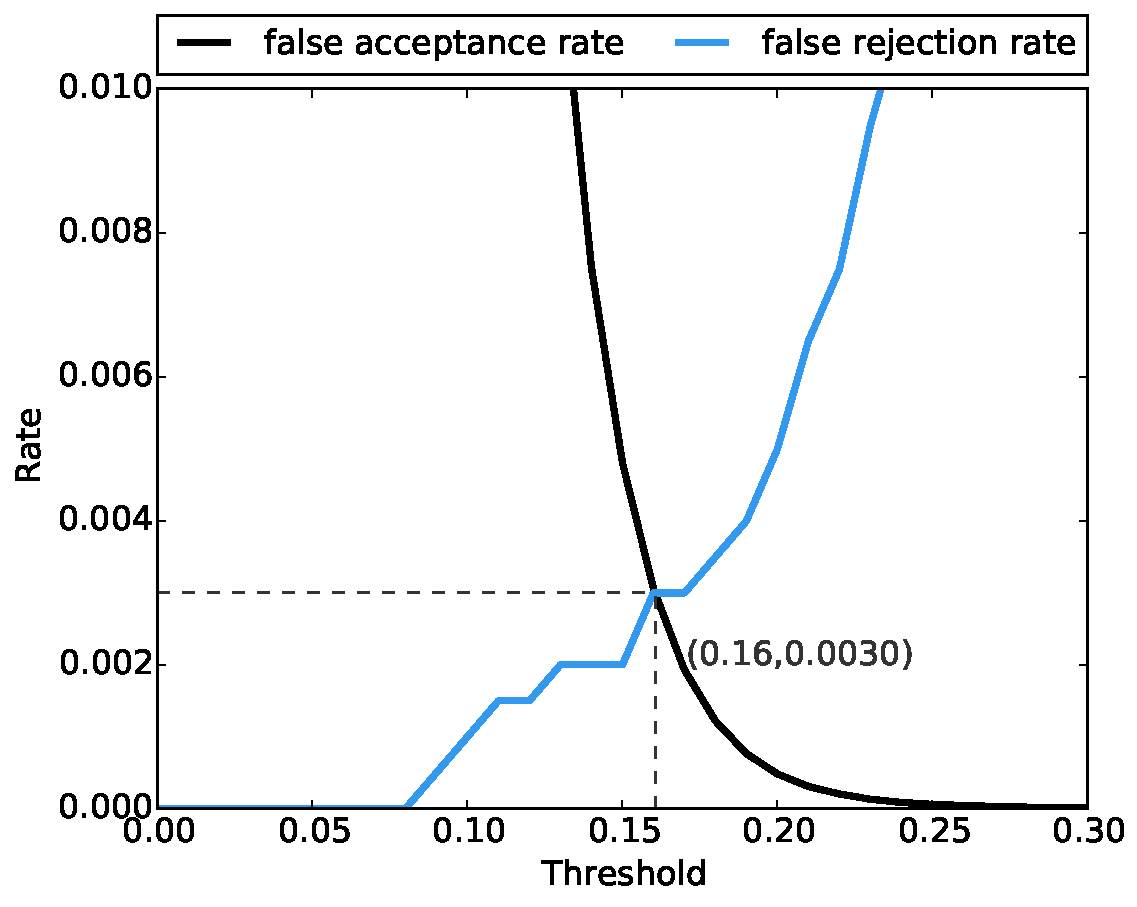
\includegraphics[width=.31\linewidth]{figures/appendix/falsepositives_80-630}}%
\subfigure[$B={[80\text{Hz}-800\text{Hz}]}$]{%
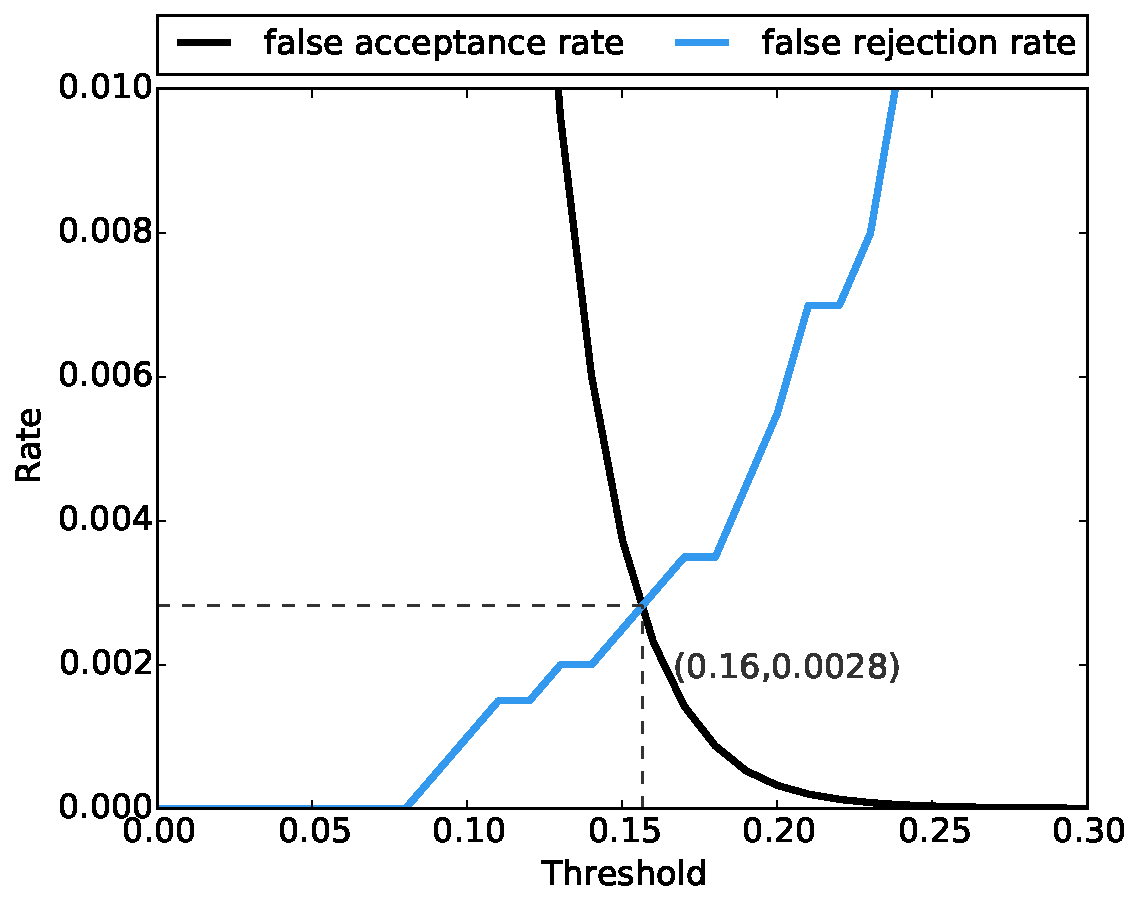
\includegraphics[width=.31\linewidth]{figures/appendix/falsepositives_80-800}}%
\subfigure[$B={[80\text{Hz}-1000\text{Hz}]}$]{%
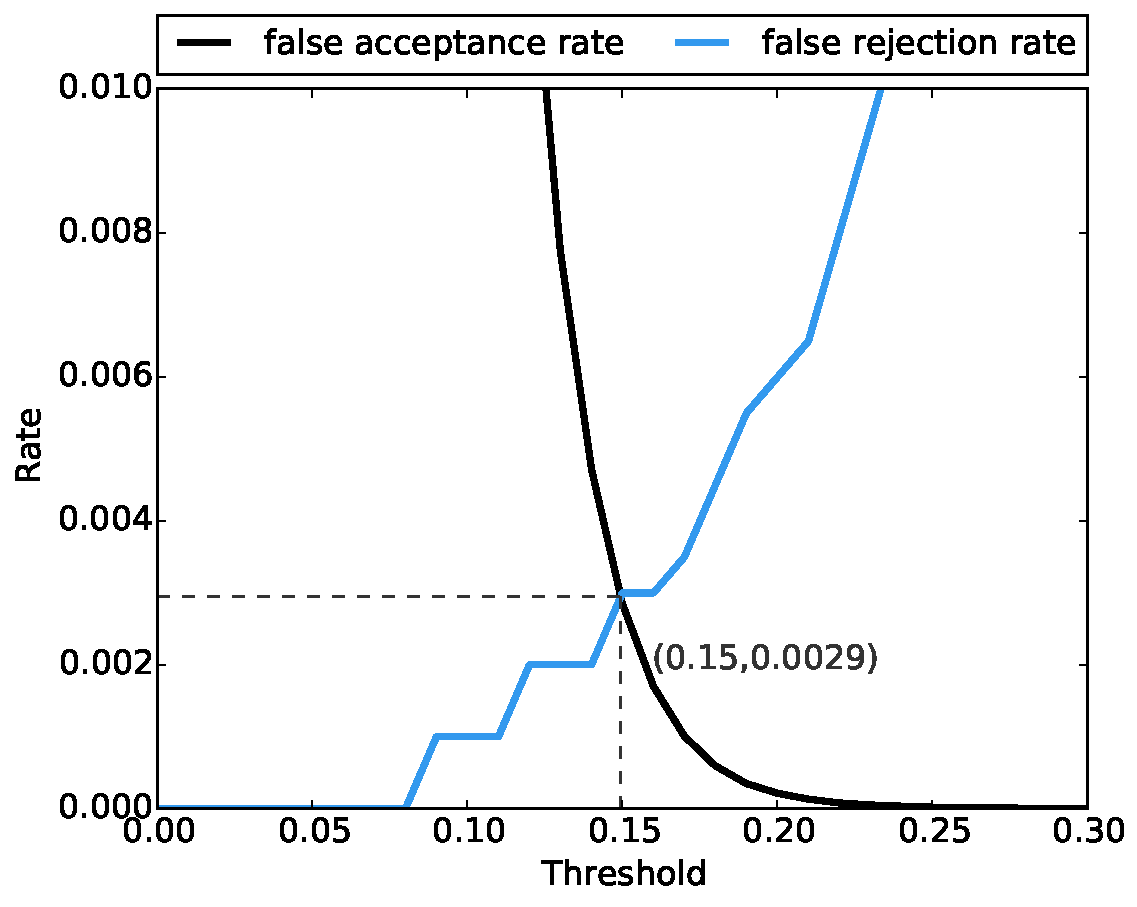
\includegraphics[width=.31\linewidth]{figures/appendix/falsepositives_80-1000}}%

\subfigure[$B={[80\text{Hz}-1250\text{Hz}]}$]{%
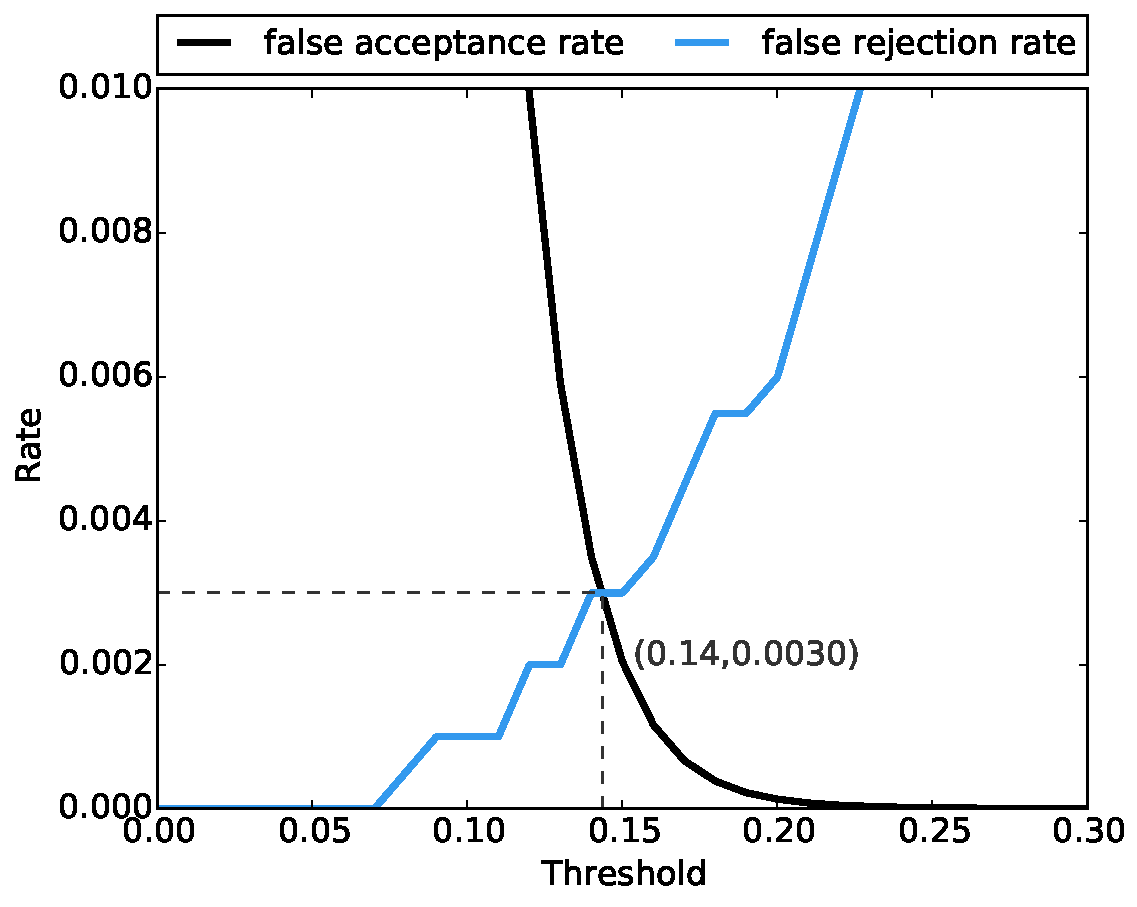
\includegraphics[width=.31\linewidth]{figures/appendix/falsepositives_80-1250}}%
\subfigure[$B={[80\text{Hz}-1600\text{Hz}]}$]{%
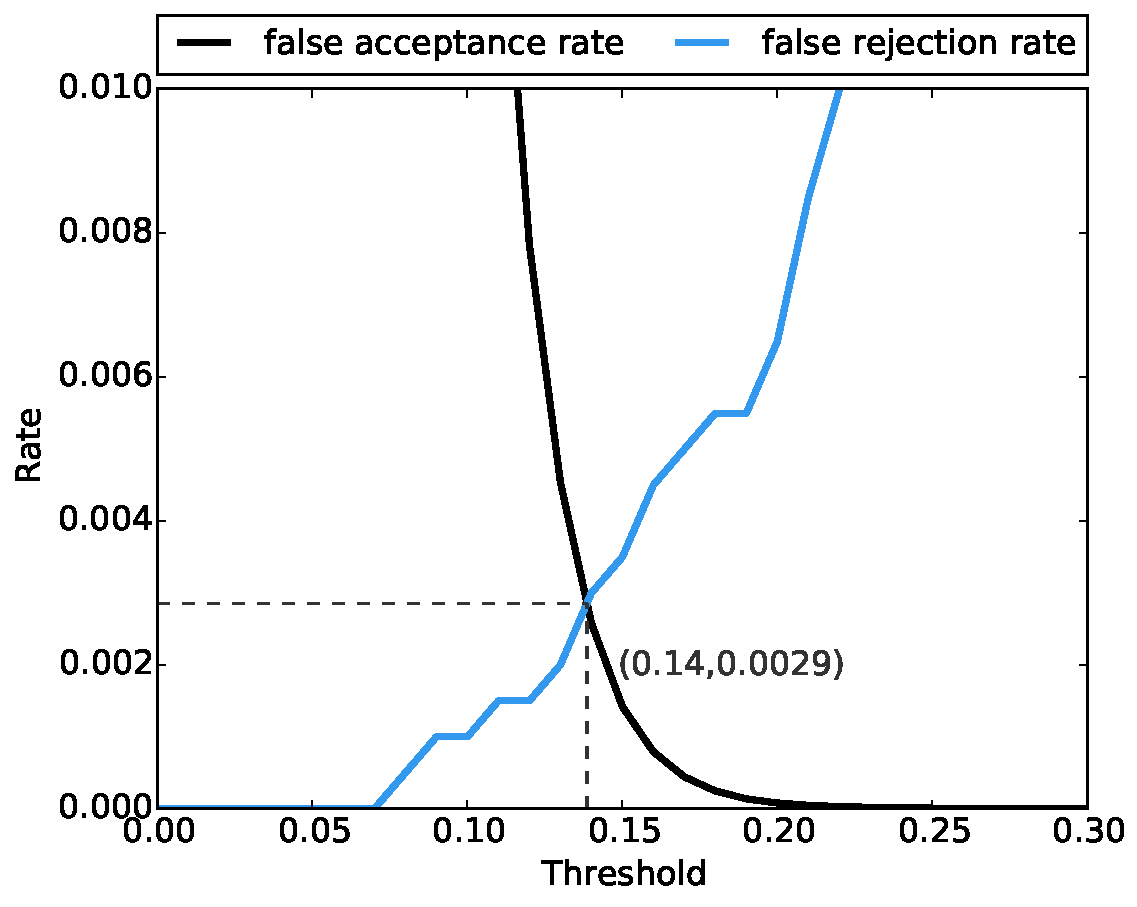
\includegraphics[width=.31\linewidth]{figures/appendix/falsepositives_80-1600}}%
\subfigure[$B={[80\text{Hz}-2000\text{Hz}]}$]{%
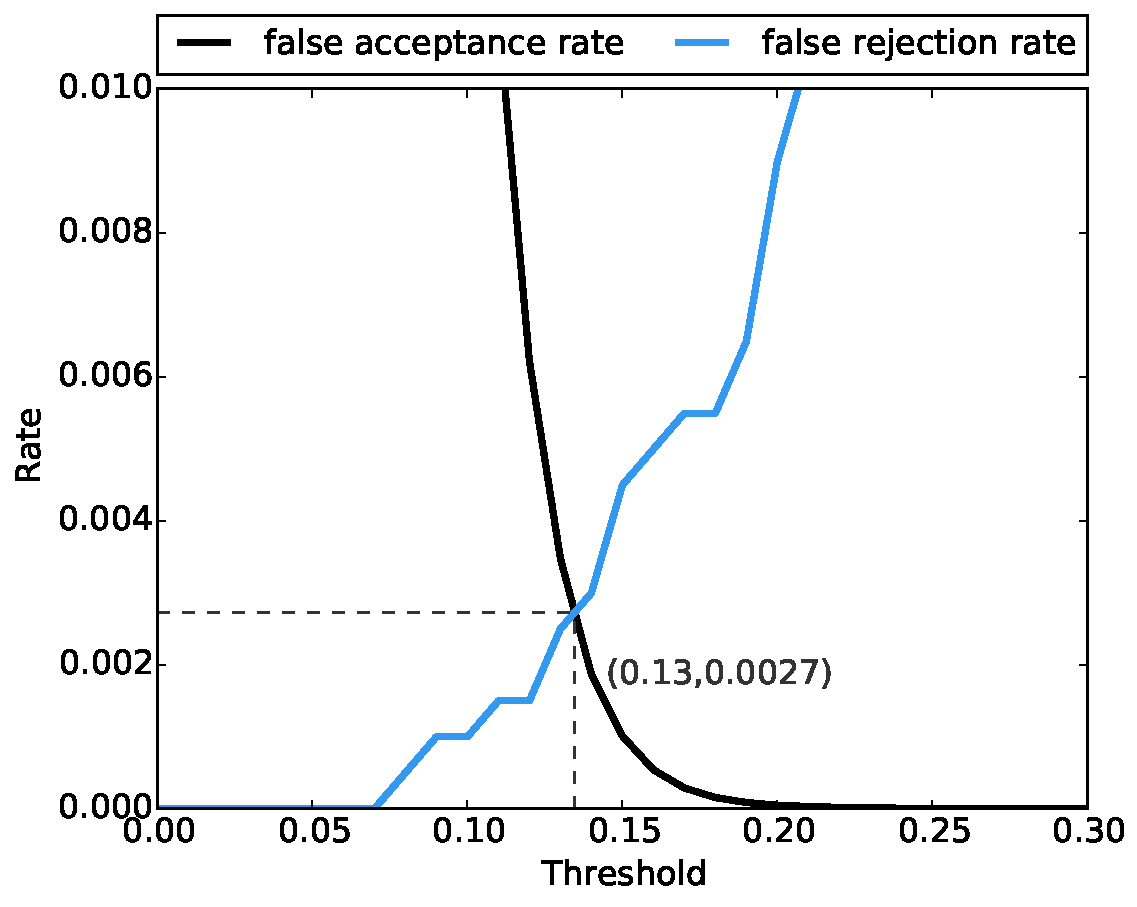
\includegraphics[width=.31\linewidth]{figures/appendix/falsepositives_80-2000}}%

\subfigure[$B={[80\text{Hz}-2500\text{Hz}]}$]{%
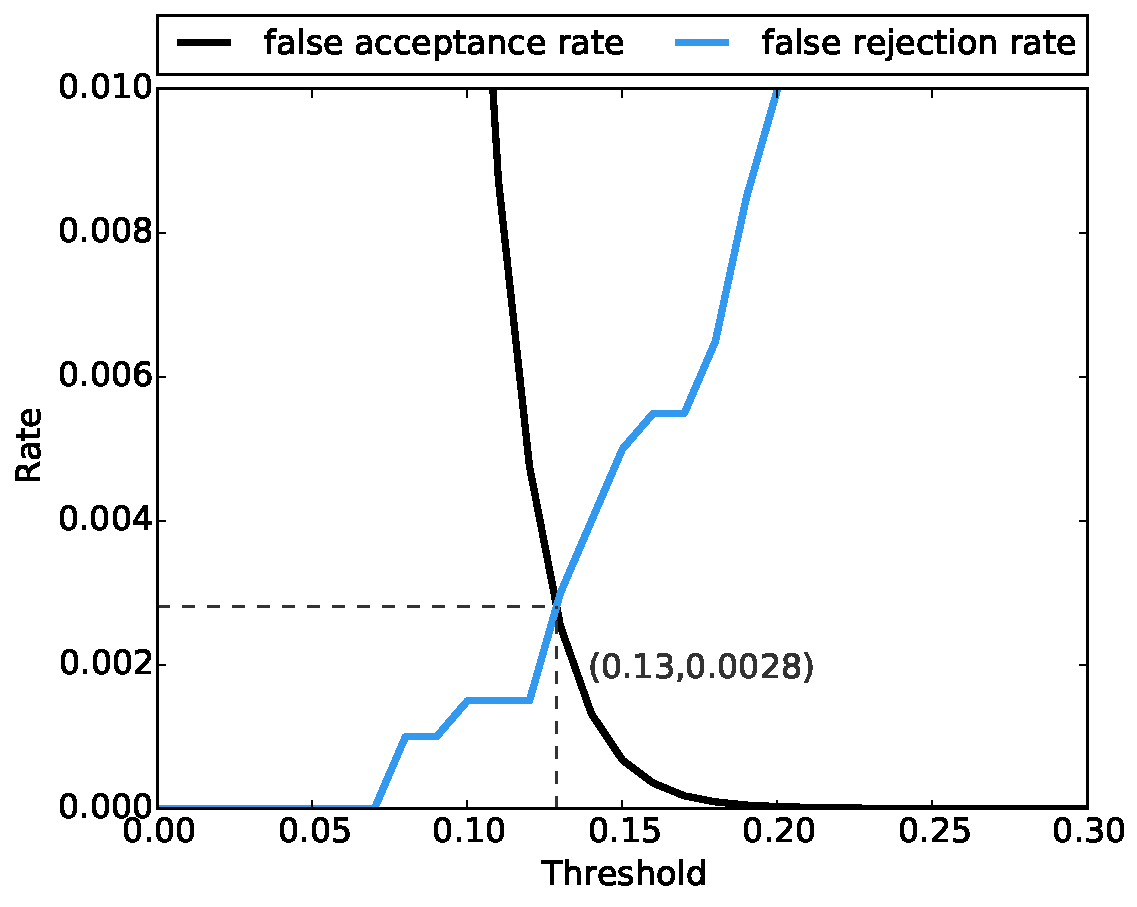
\includegraphics[width=.31\linewidth]{figures/appendix/falsepositives_80-2500}}%
\subfigure[$B={[80\text{Hz}-3150\text{Hz}]}$]{%
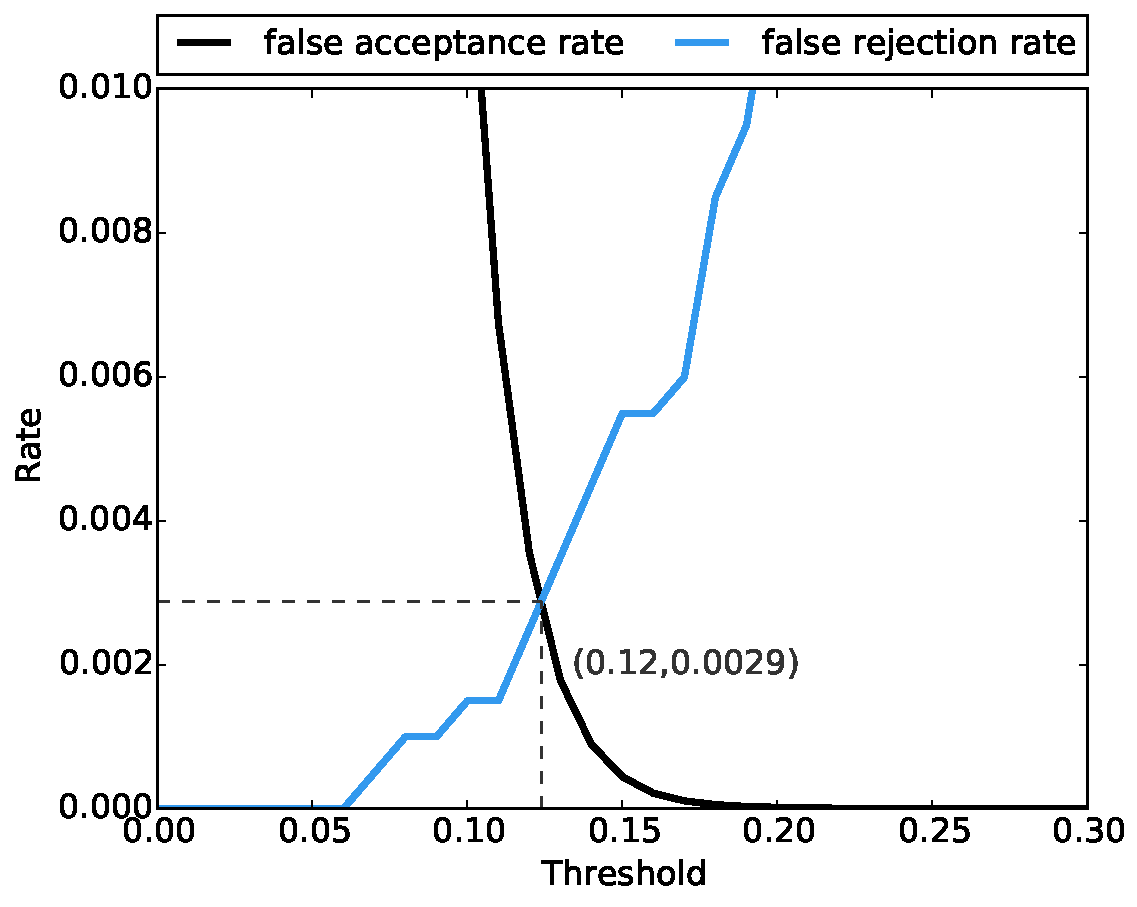
\includegraphics[width=.31\linewidth]{figures/appendix/falsepositives_80-3150}}%
\subfigure[$B={[80\text{Hz}-4000\text{Hz}]}$]{%
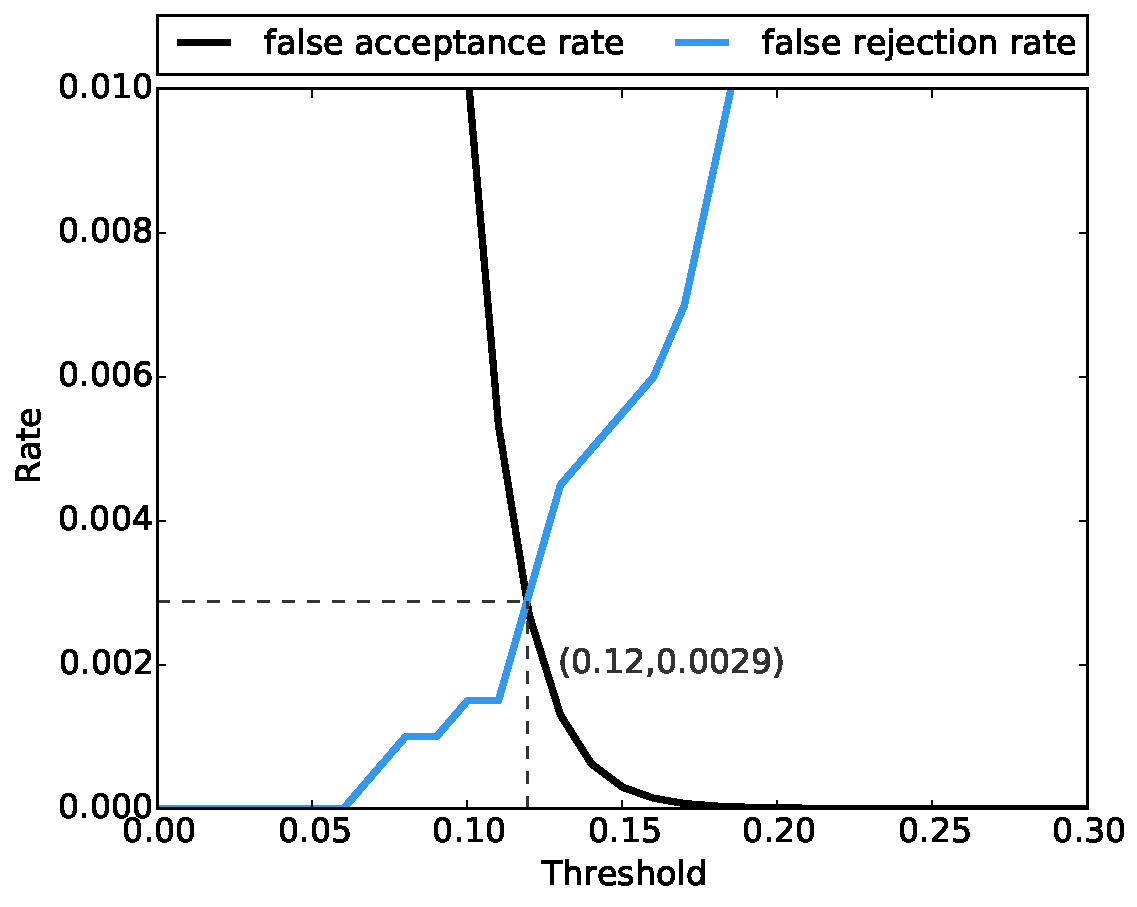
\includegraphics[width=.31\linewidth]{figures/appendix/falsepositives_80-4000}}%
\caption[{FRR and FAR as a function of the threshold $\tau_C$ for bands in the $B=[80\text{Hz}-[630\text{Hz}-4\text{kHz}]]$ range}]{False Rejection Rate and False Acceptance Rate as a function of the threshold $\tau_C$ for bands in the $B=[80\text{Hz}-[630\text{Hz}-4\text{kHz}]]$ range}
\end{figure}

\newpage

\begin{figure}[!ht]
\centering
\subfigure[$B={[100\text{Hz}-630\text{Hz}]}$]{%
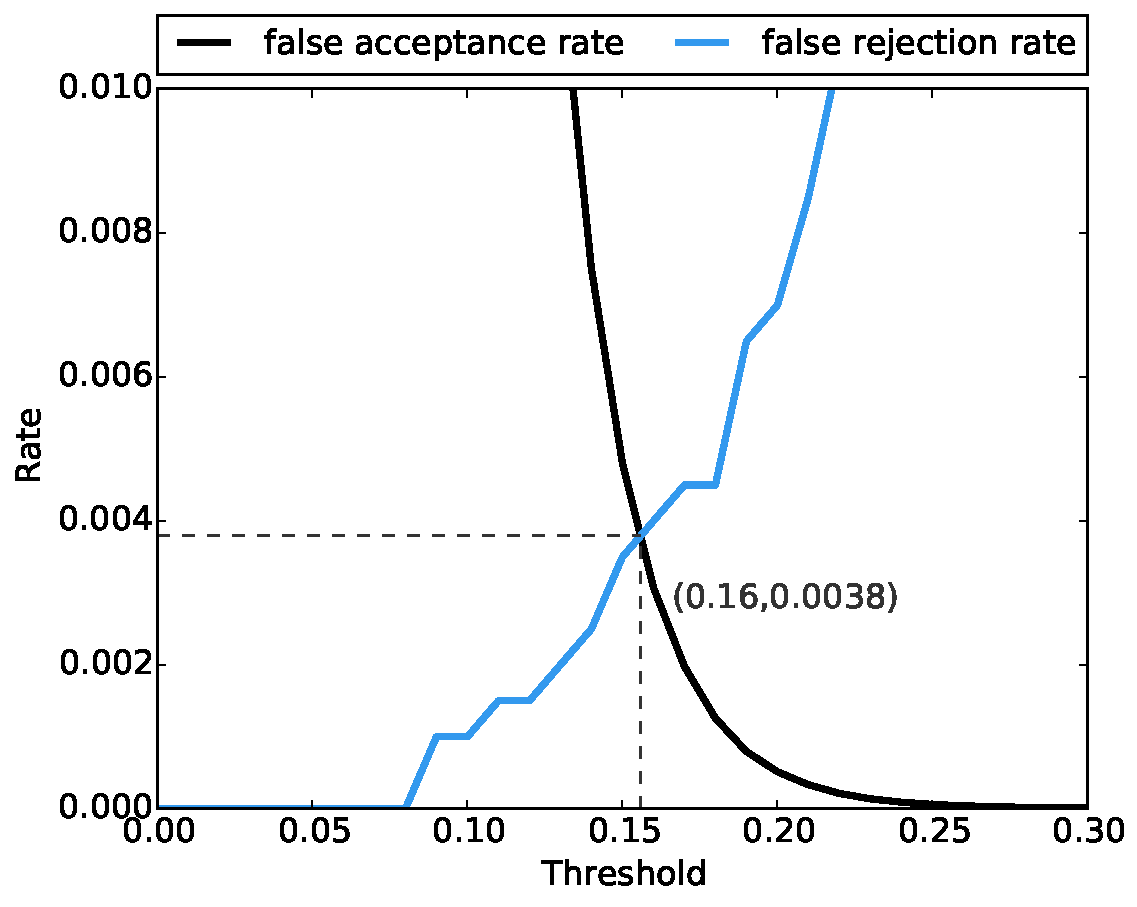
\includegraphics[width=.31\linewidth]{figures/appendix/falsepositives_100-630}}%
\subfigure[$B={[100\text{Hz}-800\text{Hz}]}$]{%
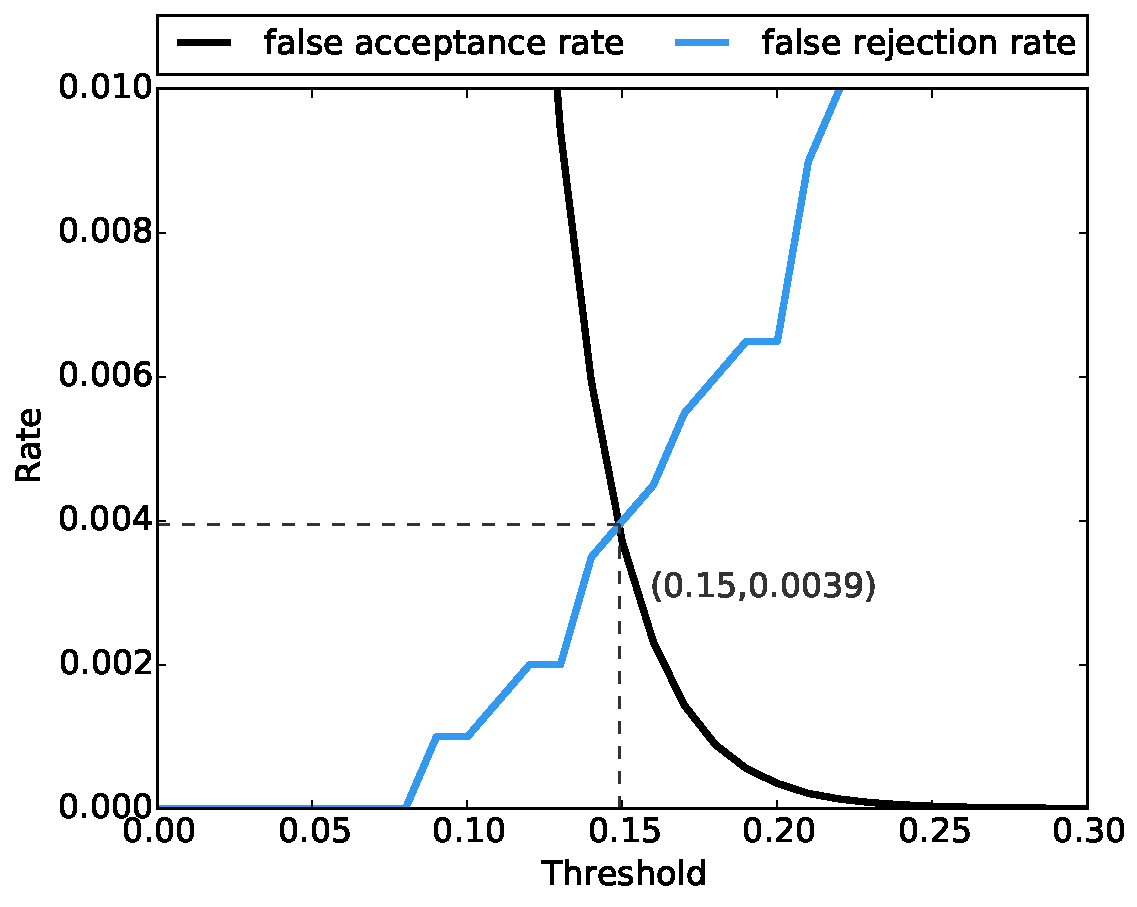
\includegraphics[width=.31\linewidth]{figures/appendix/falsepositives_100-800}}%
\subfigure[$B={[100\text{Hz}-1000\text{Hz}]}$]{%
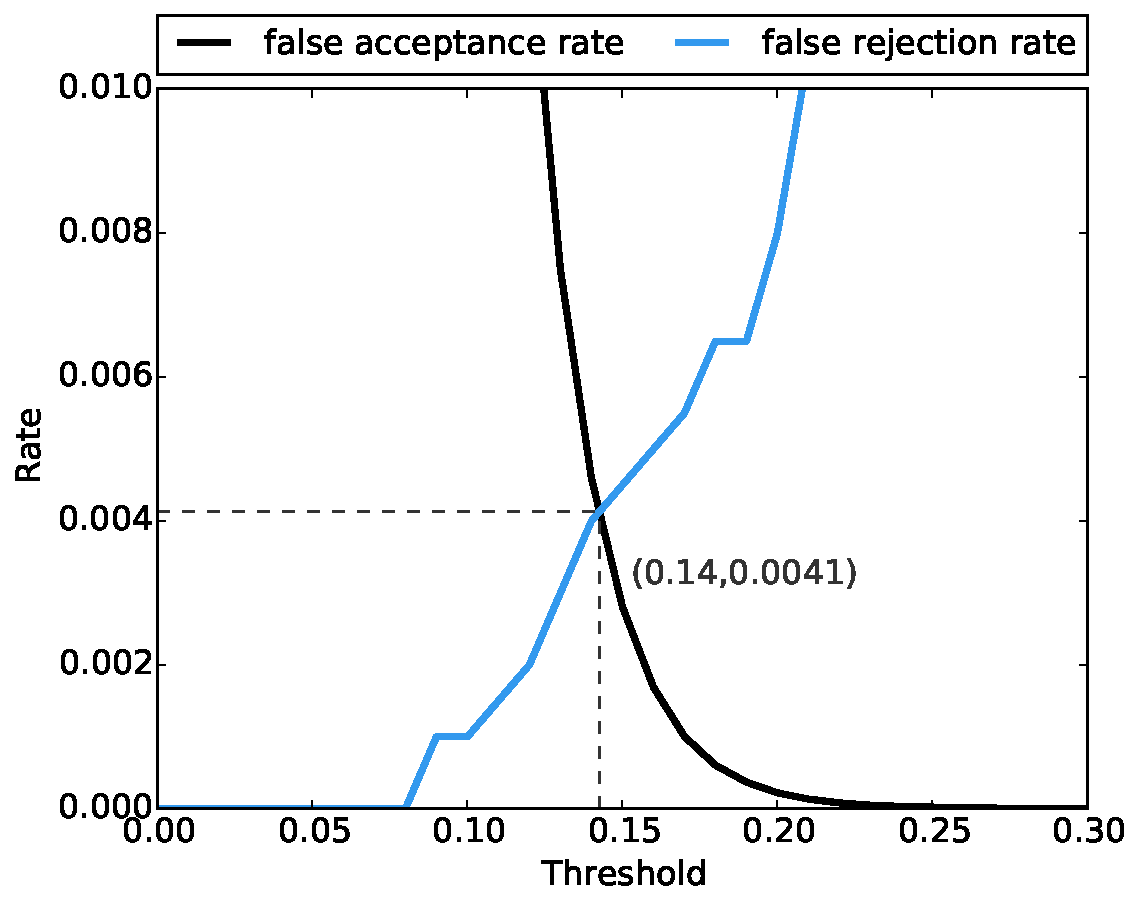
\includegraphics[width=.31\linewidth]{figures/appendix/falsepositives_100-1000}}%

\subfigure[$B={[100\text{Hz}-1250\text{Hz}]}$]{%
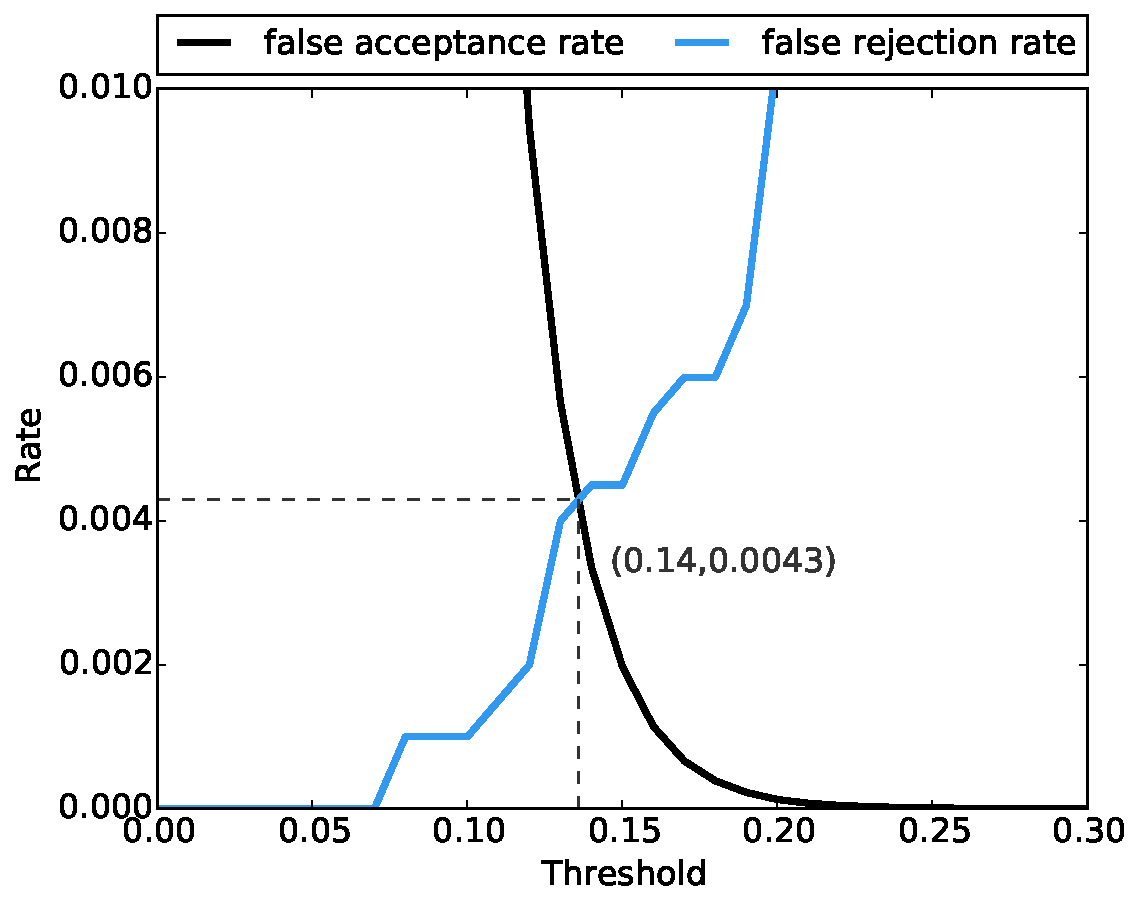
\includegraphics[width=.31\linewidth]{figures/appendix/falsepositives_100-1250}}%
\subfigure[$B={[100\text{Hz}-1600\text{Hz}]}$]{%
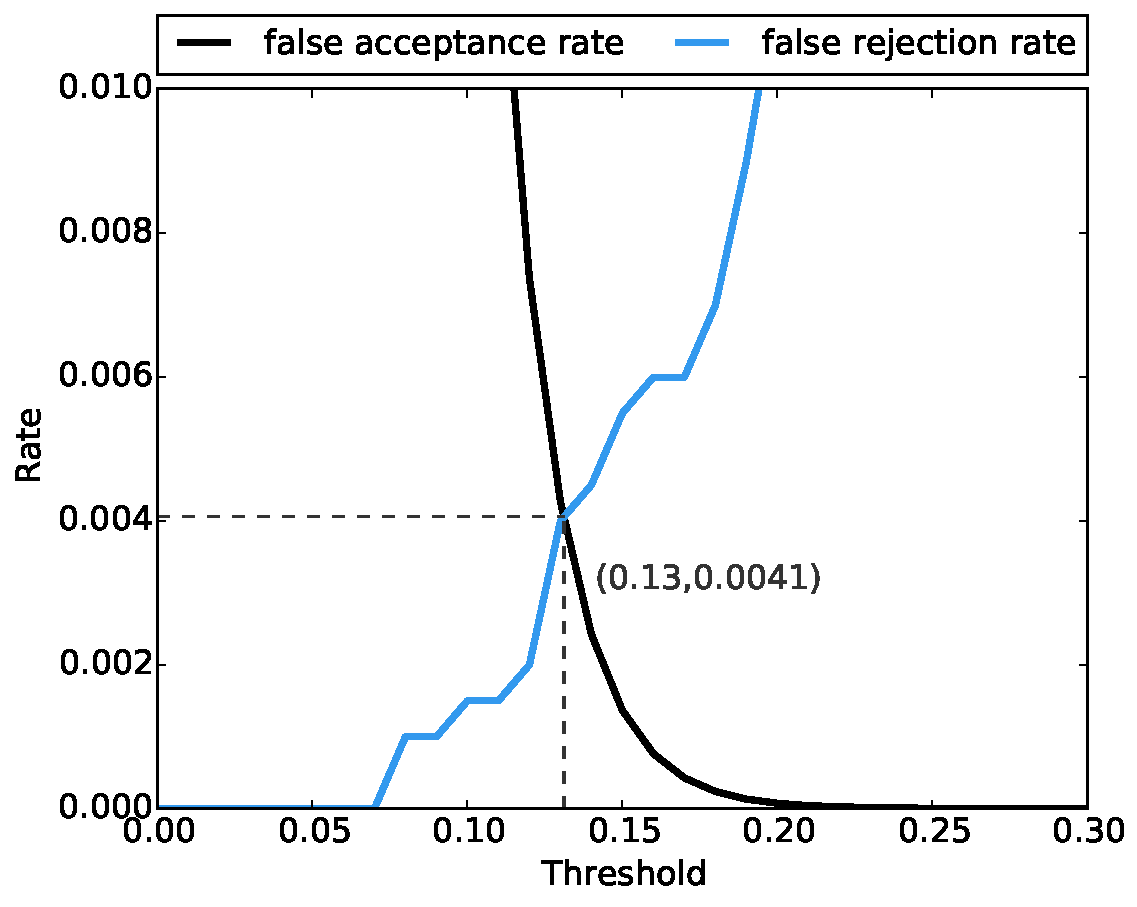
\includegraphics[width=.31\linewidth]{figures/appendix/falsepositives_100-1600}}%
\subfigure[$B={[100\text{Hz}-2000\text{Hz}]}$]{%
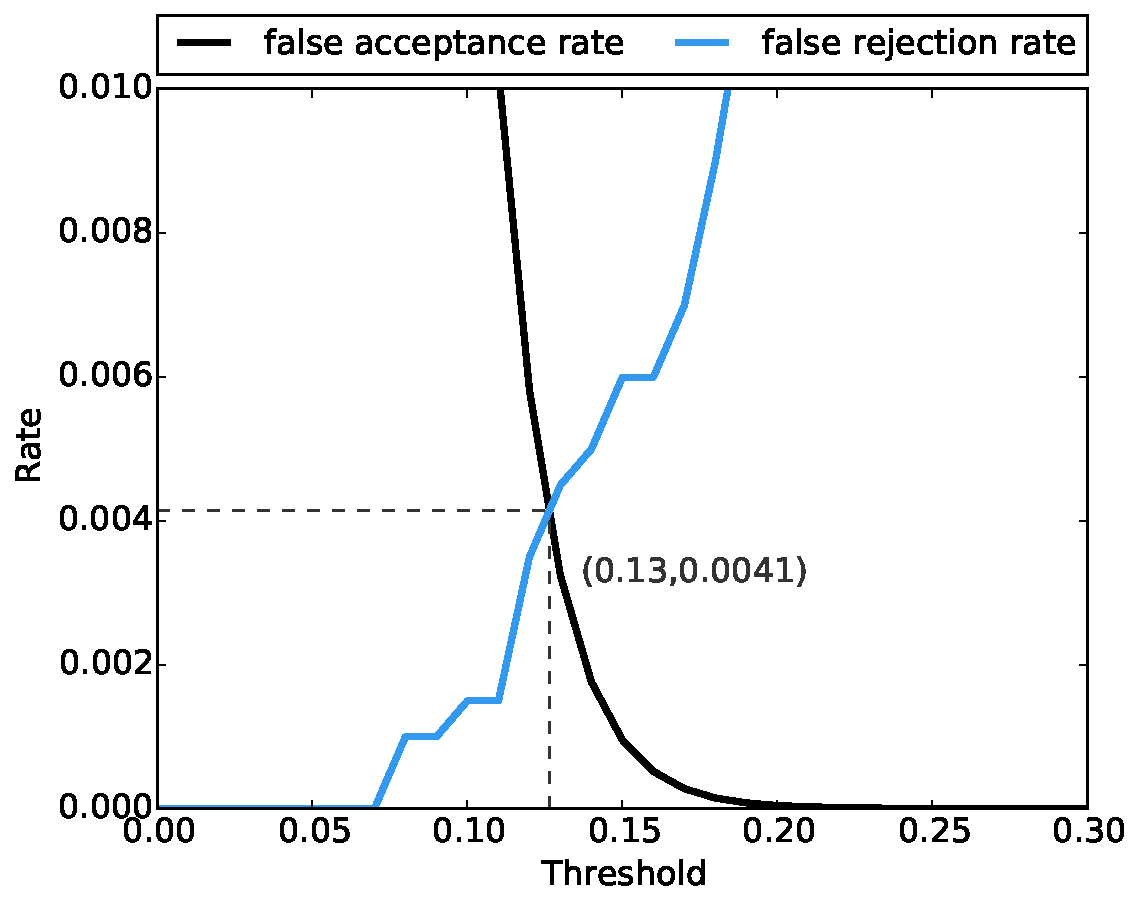
\includegraphics[width=.31\linewidth]{figures/appendix/falsepositives_100-2000}}%

\subfigure[$B={[100\text{Hz}-2500\text{Hz}]}$]{%
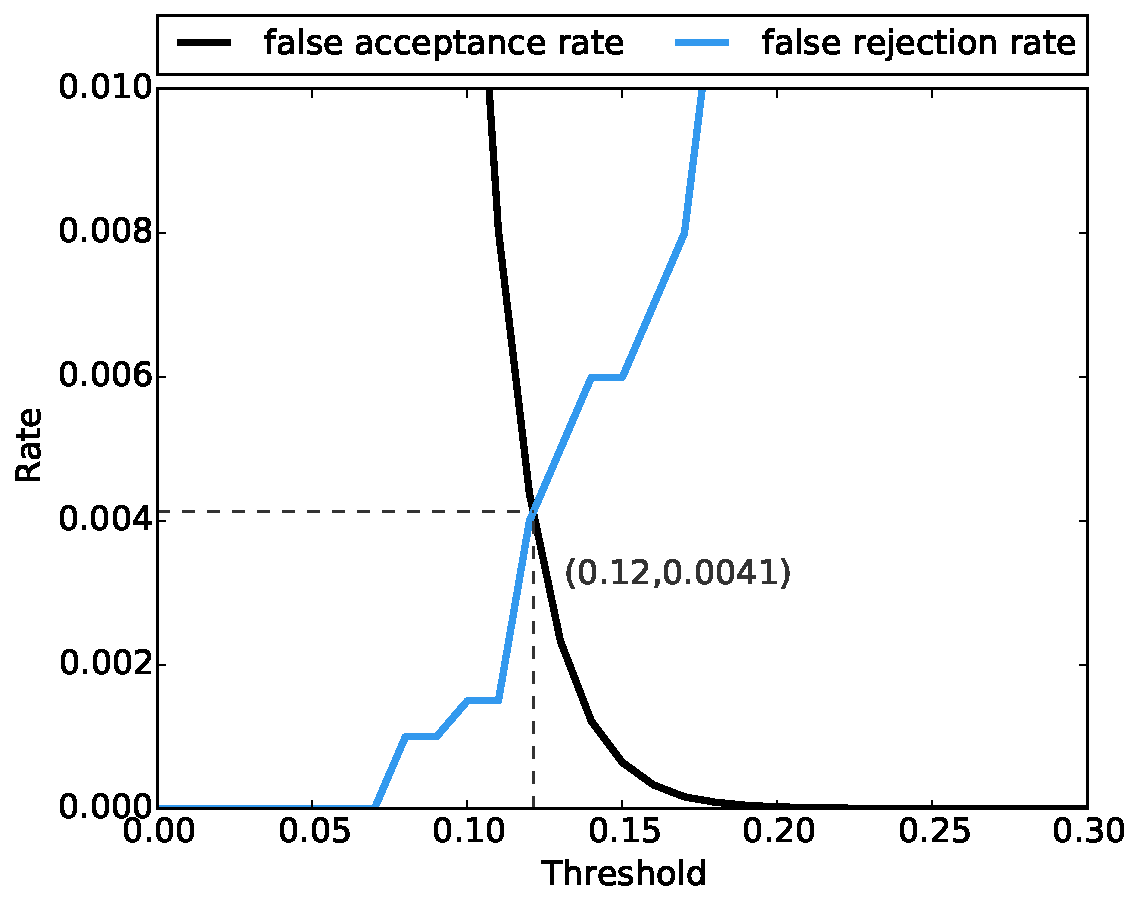
\includegraphics[width=.31\linewidth]{figures/appendix/falsepositives_100-2500}}%
\subfigure[$B={[100\text{Hz}-3150\text{Hz}]}$]{%
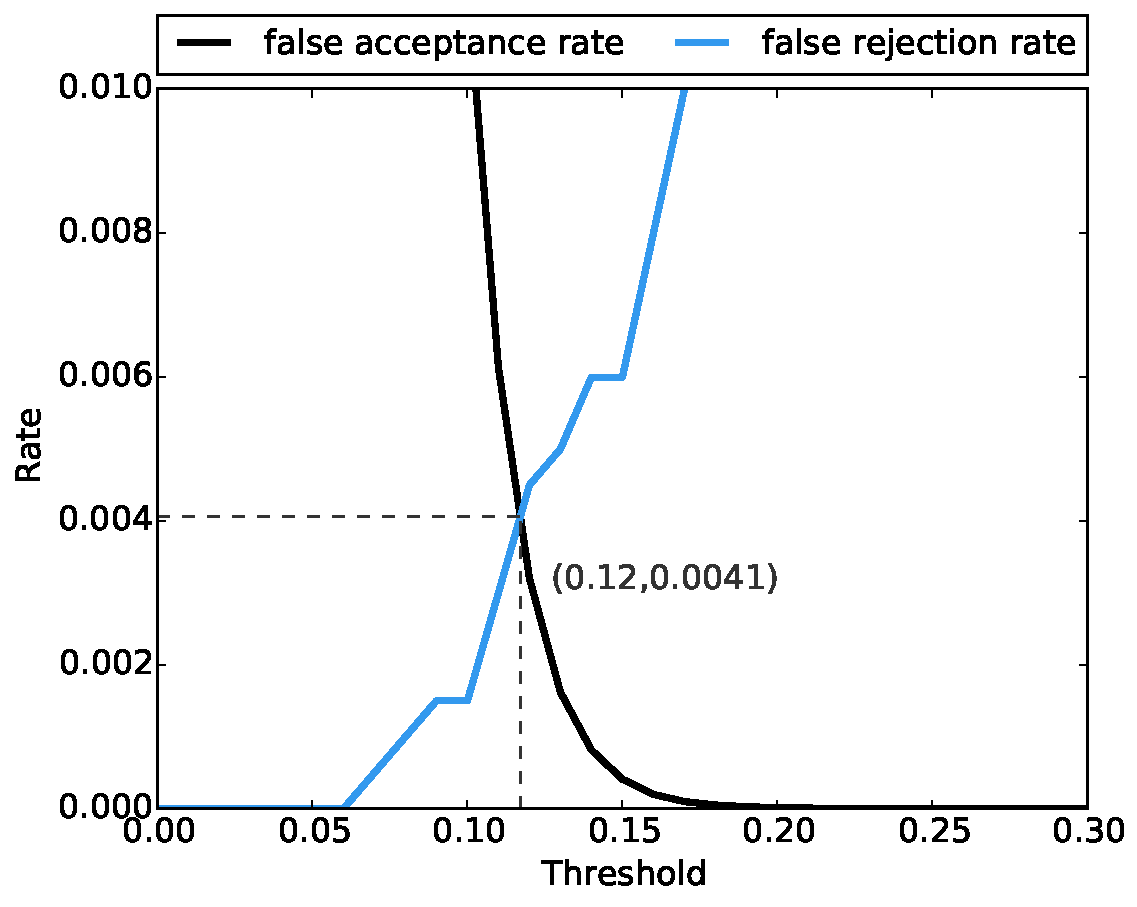
\includegraphics[width=.31\linewidth]{figures/appendix/falsepositives_100-3150}}%
\subfigure[$B={[100\text{Hz}-4000\text{Hz}]}$]{%
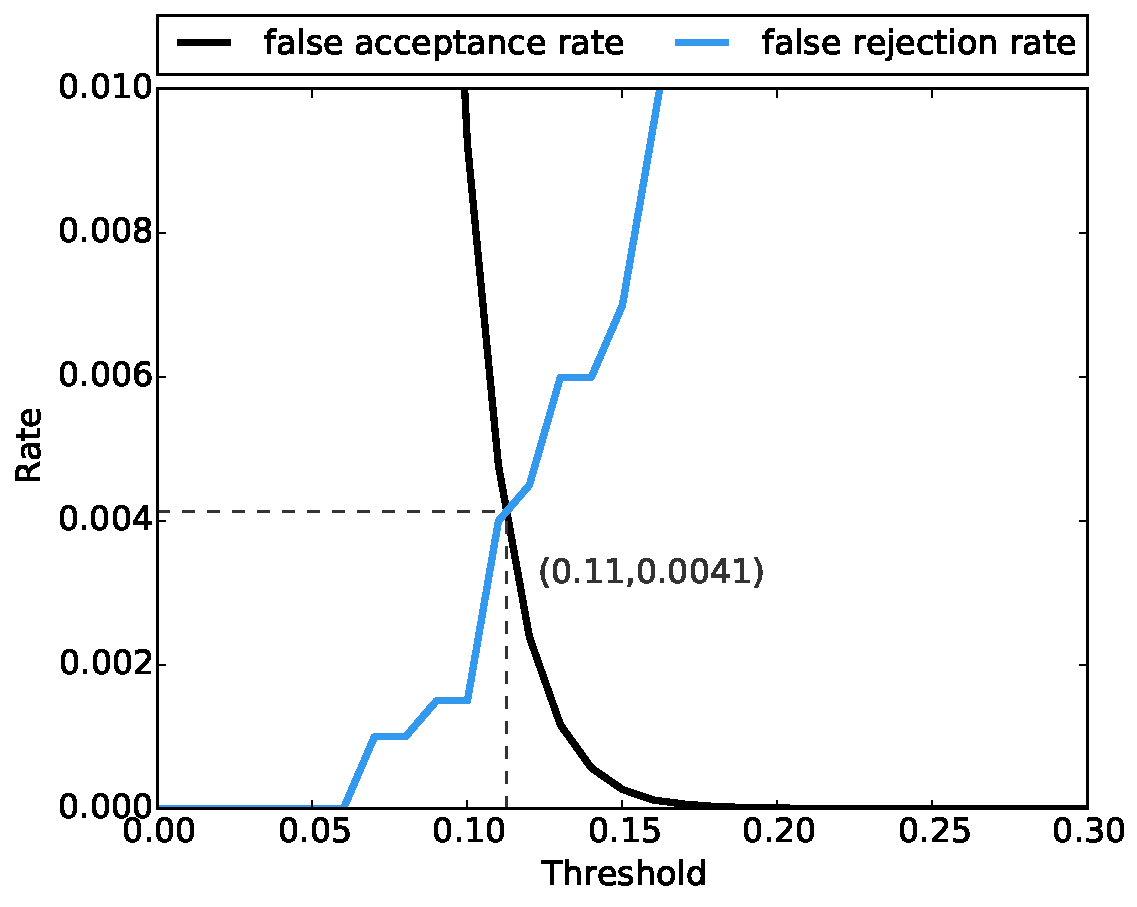
\includegraphics[width=.31\linewidth]{figures/appendix/falsepositives_100-4000}}%
\caption[{FRR and FAR as a function of the threshold $\tau_C$ for bands in the $B=[100\text{Hz}-[630\text{Hz}-4\text{kHz}]]$ range}]{False Rejection Rate and False Acceptance Rate as a function of the threshold $\tau_C$ for bands in the $B=[100\text{Hz}-[630\text{Hz}-4\text{kHz}]]$ range}
\end{figure}

\section{System Usability Scale}
\label{app:ps_sp_sus}
We report the items of the System Usability Scale~\cite{sus}.
All items were answered with a 5-point Likert-scale from \emph{Strongly Disagree} to \emph{Strongly Agree.}

\begin{itemize}[noitemsep]
\item[Q1] I think that I would like to use this system frequently.	
\item[Q2] I found the system unnecessarily complex.
\item[Q3] I thought the system was easy to use.
\item[Q4] I think that I would need the support of a technical person to be able to use this system.	
\item[Q5] I found the various functions in this system were well integrated.
\item[Q6] I thought there was too much inconsistency in this system.
\item[Q7] I would imagine that most people would learn to use this system very quickly.
\item[Q8] I found the system very cumbersome to use.
\item[Q9] I felt very confident using the system.
\item[Q10] I needed to learn a lot of things before I could get going with this system.
\end{itemize}

\section{Post-test Questionnaire}
\label{app:ps_sp_posttest}
We report the items of the post-test questionnaire.
All items were answered with a 5-point Likert-scale from \emph{Strongly Disagree} to \emph{Strongly Agree.}

\begin{itemize}[noitemsep]
\item[Q1]	I thought the audio-based method was quick.
\item[Q2]	I thought the code-based method was quick.
\item[Q3]	If Two-Factor Authentication were mandatory, I would use the audio-based method to log in.
\item[Q4]	If Two-Factor Authentication were mandatory, I would use the code-based method to log in.
\item[Q5]	If Two-Factor Authentication were optional, I would use the audio-based method to log in.
\item[Q6]	If Two-Factor Authentication were optional, I would use the code-based method to log in.
\item[Q7]	I would feel comfortable using the audio-based method at home.
\item[Q8]	I would feel comfortable using the audio-based method at my workplace.
\item[Q9]	I would feel comfortable using the audio-based method in a cafe.
\item[Q10]	I would feel comfortable using the audio-based method in a library.
\item[Q11]	I would feel comfortable using the code-based method at home.
\item[Q12]	I would feel comfortable using the code-based method at my workplace.
\item[Q13]	I would feel comfortable using the code-based method in a cafe.
\item[Q14]	I would feel comfortable using the code-based method in a library.
\end{itemize}


\section{User Comments}
\label{app:ps_sp_comments}
This section lists some of the comments that participants added to their post-test questionnaire.

\renewenvironment{quote}{%
  \list{}{%
    \leftmargin0.5cm   % this is the adjusting screw
    \rightmargin\leftmargin
  }
  \item\relax
}

\begin{quote}
``Sound-Proof is faster and automatic. Increased security without having to do more things''
\end{quote}

\begin{quote}
``I would use Sound-Proof, because it is less complicated and faster.
I do not need to unlock the phone and open the application.
In a public place it would feel a bit awkward unless it becomes widespread.
Anyway, I am already logged in most websites that I use.''
\end{quote}

\begin{quote}
``I like the audio idea, because what I hate the most about two-factor authentication is to have to take my phone out or find it around.''
\end{quote}

\begin{quote}
``Sound-Proof is much easier. I am security-conscious and already use 2FA. I would be willing to switch to the audio-based method.''
\end{quote}

\begin{quote}
``I already use Google 2SV and prefer it because I think it's more secure. However, Sound-Proof is seamless.''
\end{quote}

\section{Emails}
\label{app:sp_phishing_emails}

We reported the e-mails that were sent to participants during the duration of our user study on the effectiveness of personalized security indicators to thwart application phishing attacks.

\subsection{Advertising Email}
\label{app:sp_phishing_advertising}
We advertised a user study on the usability of a mobile banking application without mentioning any security-related feature. We also explicitly mention the duration of the user study as well as the number of tasks.

{\itshape
Dear all,

We are a research group at ETH Zurich and we are looking for participants for a new user study. We test the usability of a mobile banking application.

If you will be selected to participate, you will receive a 20.- CHF voucher redeemable at online stores (Amazon and Coop). Alternatively, participants can receive 20.- CHF cash.

Study participants should speak English and have an iPhone (model 4S,5,5S,5C,6 and iOS version 7.1 or newer).

The study will last for approximately one week during which we will ask participants to complete 4 tasks, each taking roughly 5 minutes. Participants will also fill in a pre-test and post-test questionnaires. Participants must install our test application to their iPhone.

Your identity will remain confidential and we will not collect any private data on your iPhone.
Your email address will be only used by us to contact you and will not be shared with third parties.
Should you choose to participate, you may discontinue participation at any time.

If you wish to participate, please reply to this email and we will send you further instructions. We appreciate your help!}

\subsection{Email to Selected Participants}
\label{app:sp_phishing_selectedemail}
We report the email sent to all participants that completed the pre-test questionnaire.
The email included a link to the application and the participant's credentials to access his account at SecBank.

{\itshape
Dear participant,

Thank you for participating in this user study.

In this study, you act as a customer of a fictitious bank called SecBank.
You have an account with SecBank where you have deposited fake money.
To access your account, you use a mobile banking application called ``SecBank''.

You chose SecBank as your bank because it advertises its mobile banking platform as very secure.
You want to ensure that your username and password to access your SecBank account do not fall into the wrong hands!

In the following 7 days, we will ask you to complete 4 tasks.
Each task is a mobile banking operation to be carried out with the SecBank application.
For each task, you will receive an email with detailed instructions.
To complete each task, your iPhone must be connected to the Internet.
Each task should take less than 5 minutes to complete.
We kindly ask you to complete the task within 24 hours from receiving the email.

To start off, you will need to download and install the SecBank application on your iPhone.
Username and password for your mobile banking account at SecBank are:

Username: -UNAME-\\
Password: -PWD-

The first time you start the application, please enter the email address to which you received this email: -EMAIL-

From your iPhone, visit https://www.smartphoneuserstudy.com/ to install the SecBank application.

Best regards,

Your SecBank team}

\subsection{Task Email}
\label{app:sp_phishing_taskemail}
We report the email sent to complete task number one. (Emails for the remaining tasks closely resemble this one.)

{\itshape
Dear participant,

It is time to perform the first mobile banking task with the SecBank application.

Task number 1 consists of starting the SecBank application on your iPhone and making a money transfer of \$200 to ``Anna Smith''.

The account information of ``Anna Smith'' has already been saved to the list of your favourite recipients under ``Money Transfer''.
Also we made sure that you have enough money in your account to complete the money transfer.

Once the SecBank application confirms the money transfer, the task is over.

Best regards,

Your SecBank team}


\section{Instructions for participants in the experimental groups.}
\label{app:sp_phishing_priming}

We report the priming text for participants in the experimental groups B, C and D. The paragraph was shown on the webpage where participants could download the application. The text is similar to the one provided by~\cite{boa,vanguard} to the user of their e-banking platform.

\emph{``As a major banking institution, SecBank is committed to prevent fraudulent smartphone applications from stealing your password. The SecBank mobile application uses a novel login mechanism based on personal images. The first time you login, you will be asked to pick a personal image from the photos stored in your phone. From that moment, the SecBank application will display your personal image every time it asks for your username and password. The presence of the correct personal image guarantees that you are not using a fraudulent look-alike application. You should enter your username and password only when you see your personal image. (Your personal image remains on your iPhone and is not sent to our servers.)''}

% \section{Post-test Questionnaire.}
% \label{app:sp_phishing_questionnaire}
% We report the items of the post-test questionnaire.
% All items were answered with a 5-point Likert-scale from \emph{Strongly Disagree} to \emph{Strongly Agree.}
%
% \begin{itemize}[noitemsep]
% \item[Q1] I am concerned about malware on my smartphone
% \item[Q2] I am concerned about the secrecy of my password for mobile banking
% \item[Q3] I am concerned about the secrecy of my password for my email account
% \item[Q4] I am more concerned about the secrecy of my mobile banking password compared to my email account password
% \item[Q5] During the study, I have made sure that my personal image was showing before entering my username and password
% \item[Q6] The login mechanism using personal images was intuitive and user-friendly
% \item[Q7] I would use personal images in other applications
% \end{itemize}

\section{Post-test Questionnaire: Secure Setup of Indicators}
\label{app:sp_phishing_posttestII}
We report the items of the post-test questionnaire for the user study on the indicator setup protocol (Section~\ref{sec:sp_phishing_setup}).
All items were answered with a 5-point Likert-scale from \emph{Strongly Disagree} to \emph{Strongly Agree.}

\begin{itemize}[noitemsep]
\item[Q1] The instruction sheet was clear and easy to understand
\item[Q2] The task was easy to complete
\item[Q3] I believe that I have successfully completed the task
\item[Q4] I would use this mechanism to improve the security of my mobile banking application
\end{itemize}

\newpage

\section{Bank Letter}
\label{app:sp_phishing_bankletter}

% \begin{flushright}
% \begin{tabular}{r}
% Android Bank\\
% Universit\"{a}tstrasse 6\\
% 8092 Z\"{u}rich
% \end{tabular}
% \end{flushright}
% \vspace{1cm}

\noindent\textbf{Re:} \textit{Secure set up of your personal image.}
\vspace{0.7cm}

Dear Customer,
\vspace{0.5cm}

The Android Bank application uses personal images to improve the security of its mobile banking
platform. Before using our application, you must set up a personal image.
\bigskip

\textbf{Please read carefully the instructions below and follow them to securely set up your personal image.
We advise you to read this letter until the end before starting.}
Note that during the procedure you will need the following information:

\begin{center}
{\tabulinesep=2mm
\setlength{\tabcolsep}{5mm}
\begin{tabu}{|ll|}
\hline
Service ID:     & \textbf{ax:timross}\\
PIN:            & \textbf{94455}\\
\hline
\end{tabu}}
\end{center}

\centering
\begin{tabular}{|ll|}

\end{tabular}


\noindent Instructions to securely set up your personal image.\\


\begin{enumerate}
\item Double-tap the button ``HOME'' to start the \emph{Secure Verifier} application.
\item Type in your \textbf{Service ID} and \textbf{PIN} shown above, then tap the button ``Launch Appliction''.
\item The \emph{Android Bank} application displays your PIN (\textbf{94455}). 
        \textbf{Attention!} If the PIN is \textbf{missing} or \textbf{different} from \textbf{94455}, tap the button ``HOME''.
      The installed application is not the legitimate Android Bank application.
      You \textbf{must not} select any personal image and should retain from using the application. The test is over.
\item If the PIN displayed is \textbf{identical} to your PIN (94455), tap the button ``Select Personal Image''.
        The installed application is the legitimate Android Bank application. You can safely select your personal image.
\item Select one of the images displayed and tap the button ``Confirm Selected Image''. The test is over.
\end{enumerate}

\bigskip

\hspace{8cm} Best regards,

\hspace{8.5cm} Android Bank

